% =====================================================================
%  Adaptive Chess Puzzle Advisor -- MSc Dissertation (DRAFT)
%  Structure follows the dissertation plan in the June 2026 portfolio.
%  Compile with pdfLaTeX + BibTeX (Overleaf: default settings).
% =====================================================================
\documentclass[12pt,a4paper,oneside]{report}

\usepackage[utf8]{inputenc}
\usepackage[T1]{fontenc}
\usepackage{lmodern}
\usepackage[margin=25mm]{geometry}
\usepackage{setspace}
\usepackage{graphicx}
\usepackage{booktabs}
\usepackage{tabularx}
\usepackage{array}
\usepackage{amsmath,amssymb}
\usepackage[table]{xcolor}
\usepackage{enumitem}
\usepackage{caption}
\usepackage{float}
\usepackage{url}
\usepackage[most]{tcolorbox}
\usepackage{tikz}
\usetikzlibrary{arrows.meta,positioning,fit}
\usepackage[colorlinks=true,linkcolor=blue!50!black,citecolor=green!40!black,urlcolor=blue!60!black]{hyperref}

\onehalfspacing
\setlength{\parskip}{0.4em}
\setlist{itemsep=0.2em,topsep=0.3em}
\captionsetup{font=small,labelfont=bf}
\renewcommand{\arraystretch}{1.2}
\newcolumntype{Y}{>{\raggedright\arraybackslash}X}

% ---- Draft helpers -----------------------------------------------------
% Places only the author can complete (personal reflection, supervisor
% details, ethics reference, ...). Search for "AUTHOR:" before submitting.
\newcommand{\authornote}[1]{\textcolor{red!70!black}{\textbf{[AUTHOR: #1]}}}
\newcommand{\code}[1]{\texttt{#1}}

% Headline PuzzleNet numbers (eval/neural/puzzlenet_evaluation.json),
% defined once so every chapter quotes the same value.
\newcommand{\KAPPANN}{0.91}
\newcommand{\AGREENN}{92.6\%}


% "Honest status" boxes: where the implemented work deviates from the plan.
\newtcolorbox{honest}[1][Honest status]{colback=orange!4,colframe=orange!55!black,
  fonttitle=\bfseries\small,title=#1,breakable,left=2mm,right=2mm,top=1mm,bottom=1mm}
% Key findings.
\newtcolorbox{finding}[1][Key finding]{colback=blue!3,colframe=blue!45!black,
  fonttitle=\bfseries\small,title=#1,breakable,left=2mm,right=2mm,top=1mm,bottom=1mm}

\begin{document}

\begin{titlepage}
\centering
\vspace*{15mm}
{\large City College, University of York Europe Campus\par}
{\large Department of Computer Science\par}
\vspace{25mm}
{\Huge\bfseries Adaptive Chess Puzzle Advisor\par}
\vspace{6mm}
{\Large Difficulty-Aware Bayesian Recommendation of Tactical Training\\ from Real Game Histories\par}
\vspace{25mm}
{\Large Aleksandar Radevski\par}
\vspace{6mm}
{\large MSc in Artificial Intelligence and Data Science\par}
\vspace{20mm}
{\large Supervisor: \authornote{supervisor name}\par}
\vfill
{\large October 2026\par}
\vspace{4mm}
{\small Word count: \authornote{insert final word count}\par}
\end{titlepage}

\pagenumbering{roman}
\chapter*{Abstract}
\addcontentsline{toc}{chapter}{Abstract}

Chess players improve fastest when practice targets what they actually get wrong, yet most
puzzle platforms select puzzles by rating alone. This dissertation builds and evaluates the
\emph{Adaptive Chess Puzzle Advisor}, an end-to-end system that analyses a player's Chess.com games
with Stockfish, estimates tactical weaknesses across 23 motif categories, and serves puzzles from a
5.9-million-puzzle Lichess corpus and from positions mined from the player's own games. The
recommendation core is an online Bayesian item-response model, $P(\text{solve}) =
\sigma(\theta + \delta_k - b)$, which reduces exactly to the Glicko update in one dimension. It
uses Thompson Sampling on the category offsets $\delta_k$ to choose what to practise, and sets
puzzle difficulty so that the predicted solve probability is 0.65.

Tactic labelling, which every weakness estimate depends on, is done by \emph{PuzzleNet}: a multi-task
neural network trained here on 5.5 million Lichess puzzles, which reads a position and the line that
follows it and predicts the tactical category, the theme tags, and the difficulty together with an
uncertainty. Its rating likelihood treats each puzzle's own Lichess rating deviation as known
measurement noise, so the learned variance is the uncertainty the content leaves, which is the quantity
the Bayesian recommender needs for a puzzle nobody has played.

The evaluation is deliberately adversarial to the system's own assumptions. On a held-out sample, the
hand-written tagger agrees with Lichess theme labels on 58.4\% of puzzles (Cohen's $\kappa = 0.52$),
against 31.2\% ($\kappa = 0.23$) for the original single-move labeller; PuzzleNet, scored on exactly the
same puzzles, reaches 92.6\% ($\kappa = 0.91$), and $\kappa = 0.78$ in the harder condition the
application actually runs in, labelling engine lines rather than puzzle solutions. In a pre-registered replication, the original
bandit clearly beats random selection ($d = 5.4$) but fails two of its three pre-registered
criteria. Across 200 paired simulation runs the new policy cuts puzzles the player has less than a
30\% chance of solving from 44\% to 3\%. Whether this helps learning depends on the assumed learning
mechanism. On 300 real players stratified by rating, a player's rating band is predicted from how
they play with 59.1\% accuracy (five classes, chance 20\%, permutation $p = 0.002$). However, the
tactical categories a player will miss in future games are only marginally more predictable than
population base rates, and per-category weakness shows near-zero split-half reliability --- a result
that survives relabelling every one of those players' 40{,}067 critical positions with the neural
labeller, so it is not an artefact of crude labels.

The central conclusion is that the robust contribution is \emph{adaptive difficulty}, and that
personal tactical weaknesses are too subtle to diagnose from typical game histories and must be
learned online from targeted puzzle attempts. The generative-RL puzzle creation and human
evaluation envisaged in the project plan were not carried out. Both are discussed, with a
pre-registered study protocol for the latter.

\vspace{4mm}
\noindent\textbf{Keywords:} Thompson Sampling, item response theory, Glicko-2, adaptive learning,
chess tactics, player modelling, multi-task neural networks, heteroscedastic regression, simulation study.

\chapter*{Declaration}
\addcontentsline{toc}{chapter}{Declaration}

\authornote{Replace this chapter with the declaration wording required by City College. The text
below is a draft.}

I declare that this dissertation is my own work, that it has not been submitted for any other
degree or qualification, and that all sources are acknowledged.

\section*{Use of generative AI tools}

\authornote{Adapt this statement to City College's policy on AI tools, and describe your actual use
accurately. Examiners may ask about it in the viva.}

Generative AI assistance (Anthropic's Claude, via Claude Code) was used during this project for:
\begin{itemize}
  \item writing and refactoring parts of the software, including the recommendation models, the
        tactic tagger, and the evaluation and data-collection scripts;
  \item designing and running the simulation study and the statistical analyses;
  \item checking references against publisher records;
  \item producing a first draft of the structure and text of this document.
\end{itemize}
All design decisions, results and conclusions were reviewed by the author, who takes
responsibility for them. The prose has been \authornote{describe how you revised or rewrote the
draft text in your own words}.

\section*{Data and ethics}

The research cohort in Chapter~6 consists of publicly available Chess.com games collected through the
Chess.com Published-Data API. Players are stored under salted pseudonyms, and only aggregate
statistics are reported. The ethics position of this use is \authornote{state the ethics approval
reference, or the supervisor's confirmation that no approval was required}.

\chapter*{Acknowledgements}
\addcontentsline{toc}{chapter}{Acknowledgements}

\authornote{Thank your supervisor, the players who used the app, and anyone else who helped.}


\tableofcontents
\listoffigures
\listoftables
\clearpage
\pagenumbering{arabic}

\chapter{Introduction}\label{ch:intro}

\section{Background and Motivation}

Chess is no longer only a board game. It has become a large-scale testbed for artificial
intelligence, from hand-crafted alpha-beta searchers to self-taught reinforcement-learning systems
such as AlphaZero~\cite{silver2018general}. Online platforms record hundreds of millions of games
every year, and open databases such as the Lichess puzzle collection~\cite{lichessdb} turn that
activity into millions of rated training positions. For the first time, the way ordinary club
players make decisions can be studied statistically, at scale.

The most popular training tool on these platforms is the tactical puzzle: a position with a single
clearly best continuation, which the player must find. Research on expertise suggests that practice
is effective in proportion to how precisely it targets a learner's current deficiencies, and that
repeating skills that are already mastered adds little~\cite{ericsson1993role}. Puzzle platforms,
however, mostly select puzzles by \emph{rating}. A player who handles forks well but repeatedly
misses back-rank mates still receives mostly forks, because forks are common. The practice is
comfortable, and largely redundant.

The original motivation for this project, as set out in the portfolio, was more ambitious. It was to
recognise a player's style of play (positional, attacking, defensive) from their move sequences,
and to generate new puzzles for that player based on the mistakes in their recent games. Over the
course of the project the emphasis shifted, in response to evidence gathered along the way, from
\emph{style} and \emph{generation} towards \emph{diagnosis} and \emph{adaptive selection}: finding
out what a player gets wrong, and serving the right puzzle at the right difficulty.
Section~\ref{sec:scope} documents this shift explicitly.

\section{Problem Statement}

Given a player's recent game history and a large pool of candidate puzzles, choose a sequence of
puzzles that maximises training value for that player. Four difficulties make this hard:

\begin{enumerate}
  \item \textbf{Weakness is not directly observable.} It must be inferred from noisy binary
        evidence (a puzzle is solved or not; a critical move in a game is found or missed), and every
        observation costs the learner time.
  \item \textbf{Tactic labels are noisy.} Deciding automatically \emph{which} motif a missed move
        belongs to is itself an unsolved classification problem.
  \item \textbf{Difficulty scales do not match.} A player's game rating on Chess.com and a puzzle's
        rating on Lichess are different scales, so ``puzzles near your rating'' is poorly defined.
  \item \textbf{Data per player is scarce.} A typical analysis covers about 50 games and roughly 80
        critical positions, spread across more than a dozen tactical categories.
\end{enumerate}

\section{Aim and Research Objectives}

The aim stated in the portfolio was \emph{``to design and evaluate an adaptive puzzle generator for
chess puzzles that helps players to enhance their skills by using reinforcement learning and player
style classification.''} The four objectives, and their status at the time of writing, are listed
in Table~\ref{tab:objectives}.

\begin{table}[H]
\centering
\small
\caption{Portfolio objectives and their status.}\label{tab:objectives}
\begin{tabularx}{\linewidth}{p{0.3\linewidth}Yp{0.13\linewidth}}
\toprule
\textbf{Objective (portfolio wording)} & \textbf{What was done} & \textbf{Status} \\
\midrule
O1. A classification model that predicts player rating group or style from gameplay data, with
statistically significant performance on unseen players. &
Rating-band classifier on 300 real players, cross-validated over players: 59.1\% accuracy over five
bands (chance 20\%), permutation $p=0.002$ (Section~\ref{sec:rating-classifier}). Style is covered
only by a rule-based archetype heuristic. & Met (rating group); style not met \\
O2. An adaptive puzzle generator that creates legal, unique and novel puzzles, optimised for
counter-intuitiveness and realism. &
Engine-verified \emph{mining} of puzzles from the player's own games through four Stockfish gates
(legal and unique by construction), plus a 5.9M-puzzle Lichess pool. No generative model, and no
counter-intuitiveness optimisation. & Partially met (reframed) \\
O3. A difficulty-matching module that selects puzzles according to player strength and prior
interaction history. &
An online Bayesian IRT learner that pitches each puzzle at a predicted 65\% solve probability, per
category, updated after every attempt (Section~\ref{sec:rl-setup}). & Met \\
O4. Evaluation with automatic puzzle-quality metrics and human assessment, showing improved fit
compared with a non-adaptive baseline. &
Automatic metrics, a pre-registered replication, a paired simulation study (seven experiments) and a
300-player real-data evaluation. The human study is designed but has not been run. & Partially met \\
\bottomrule
\end{tabularx}
\end{table}

\section{Research Questions}

The objectives lead to five research questions, each answered in Section~\ref{sec:answers}:

\begin{description}
  \item[RQ1] Can a player's rating group be predicted from \emph{how} they play, on players the model
        has never seen, without access to any rating information? (O1)
  \item[RQ2] Can a player's tactical weaknesses be diagnosed from their game history reliably
        enough to personalise training? (O1, O3)
  \item[RQ3] How reliably can the tactical motif of a position be labelled automatically, and does
        label quality matter downstream? (O2)
  \item[RQ4] Does difficulty-aware adaptive selection match puzzles to the player better than a
        fixed rating band? (O3)
  \item[RQ5] Does adaptive selection outperform non-adaptive baselines, and under which
        assumptions? (O4)
\end{description}

\section{Scope and Assumptions}\label{sec:scope}

\begin{honest}[Honest status: deviations from the portfolio plan]
\begin{itemize}
  \item \textbf{No generative model or RL fine-tuning of puzzles was built.} The portfolio's
        research gap, ``style- and rating-aware puzzle generation from scratch using generative RL
        conditioned on the learner'', remains open. The comparable published system (Feng et
        al.~\cite{feng2025generating}) pre-trains on 4.4 million puzzles and fine-tunes with RL at
        industrial-lab scale. Puzzles here are \emph{mined} from real games and verified by engine,
        so ``novel'' means novel \emph{to the player}, not new to the world.
  \item \textbf{Style classification was not built as a machine-learning model.} Objective O1 is met
        through the alternative the portfolio allowed, the \emph{rating group}.
  \item \textbf{No human assessment has yet been carried out.} Chapter~\ref{ch:discussion} and
        Appendix~\ref{app:repro} refer to a pre-registered protocol with a power analysis (34 paired
        participants are needed to detect a medium effect).
\end{itemize}
\end{honest}

\noindent\textbf{Assumptions.}
\begin{itemize}
  \item Stockfish~\cite{stockfish} at the node budgets used here (75,000 nodes per position for game
        analysis, depth 18 for puzzle verification) is treated as ground truth for move quality.
  \item Lichess puzzle themes are treated as a \emph{reference} for tactic labels. They are produced
        by an automatic tagger themselves, so agreement is not the same as accuracy.
  \item The probability of solving a puzzle follows a logistic (Rasch-type) form in the gap between
        ability and difficulty, as Elo and Glicko also assume~\cite{elo1978rating,glickman1999parameter}.
  \item Publicly available Chess.com games may be analysed for research when they are pseudonymised
        and reported only in aggregate (see the Declaration).
\end{itemize}

\section{Contributions of the Dissertation}

\begin{enumerate}
  \item \textbf{A working end-to-end system.} It covers Chess.com ingestion, deterministic Stockfish
        analysis graded by win probability, critical-position (opportunity) logging, weakness
        profiling, puzzle mining and adaptive serving, delivered as a Flask web application with 231
        offline tests.
  \item \textbf{A difficulty-aware Bayesian recommender.} An online item-response learner with a
        full-covariance Laplace update that reduces exactly to Glicko's update in one dimension
        (tested to $10^{-9}$). It combines Thompson Sampling over per-category ability offsets with
        per-puzzle difficulty targeting.
  \item \textbf{A validated line-level tactic tagger.} On a held-out sample, agreement with Lichess
        themes rises from 31.2\% ($\kappa=0.23$) to 58.4\% ($\kappa=0.52$).
  \item \textbf{PuzzleNet, a multi-task neural model of tactic and difficulty.} A network trained on
        5.5M Lichess puzzles that reads a position and the line that follows it and predicts the
        tactical category, the theme tags, and the difficulty \emph{with an uncertainty}. The rating
        likelihood treats each puzzle's Lichess rating deviation as known measurement noise, so the
        learned variance carries only what the content leaves uncertain, and that variance is then
        consumed directly by the Bayesian recommender as a puzzle's difficulty uncertainty. On the same
        held-out puzzles as the rule-based tagger, agreement rises to \AGREENN{} ($\kappa=\KAPPANN{}$), and
        mined puzzles gain a calibrated difficulty estimate in place of a closed-form guess. The network,
        its gradients and its optimiser are implemented from first principles in NumPy and checked
        against finite differences.
  \item \textbf{A rigorous comparative evaluation.} A pre-registered replication (reported
        including its failures), seven paired simulation experiments with Holm-corrected tests, and a
        prequential calibration on real solve logs.
  \item \textbf{A 300-player real-data evaluation.} Rating group is predictable from play; per-category
        weakness is almost entirely noise at typical data volumes; the rule-based and
        synthetic-trained profilers carry no predictive information.
  \item \textbf{Population category norms} fitted on the cohort. They separate ``this motif is hard for
        everyone'' from ``this player is weak at it''.
  \item \textbf{Documented engineering defects and fixes.} Several defects silently disabled or
        corrupted parts of the system; they are reported in Section~\ref{sec:challenges} because they
        bear on the validity of earlier results.
\end{enumerate}

\section{Dissertation Outline}

Chapter~\ref{ch:literature} reviews computer chess, puzzle platforms, player modelling, generative
models and RL, and difficulty modelling. Chapter~\ref{ch:problem} formalises the problem and presents
the system architecture. Chapter~\ref{ch:method} describes the methodology, and
Chapter~\ref{ch:implementation} the implementation. Chapter~\ref{ch:results} reports the experiments.
Chapter~\ref{ch:discussion} discusses the findings, including an honest assessment of how
sophisticated the AI in this system is. Chapter~\ref{ch:conclusion} answers the research questions
and recommends future work.

\chapter{Background and Literature Review}\label{ch:literature}

\section{Chess Engines and Computer Chess}

Classical chess engines combine alpha-beta search with an evaluation function. The landmark
1997 match in which IBM's Deep Blue defeated Garry Kasparov showed that hand-crafted evaluation
combined with massive search could beat the world champion. Modern engines retain that search
architecture but have replaced the hand-written evaluation. Stockfish~\cite{stockfish}, the
strongest open-source engine, evaluates positions with an \emph{efficiently updatable neural
network} (NNUE), originally developed for computer shogi by Nasu~\cite{nasu2018nnue}. Because the
network's first layer can be updated incrementally as pieces move, a neural evaluation becomes
cheap enough to run inside a search visiting millions of positions per second. That property
matters for this dissertation, which analyses about 18,000 games.

A second line of work replaces search heuristics with learning altogether. AlphaZero learns a
policy and a value function by self-play and combines them with Monte Carlo tree search, reaching
superhuman strength from the rules alone~\cite{silver2017mastering,silver2018general}. Zahavy et
al.~\cite{zahavy2023diversifying} show that a single AlphaZero policy is near-optimal but narrow. It
fails on out-of-distribution positions, such as Penrose-style puzzles that are easy for humans.
Their AZdb system trains a population of latent-conditioned policies with diversity bonuses; it
solves more hard puzzles and plays in more varied styles.

These systems are designed to \emph{play} well. Maia~\cite{mcilroyyoung2020aligning} takes the
opposite view: it trains networks on human games to predict the move a human \emph{of a given
rating} would play, rather than the best move. For a training system this distinction is central.
The engine tells us what is correct; a human-behaviour model would tell us what a particular player
is likely to find. This dissertation uses Stockfish as an oracle of correctness. Maia-based
difficulty estimates are discussed as future work (Section~\ref{sec:future}).

\section{Chess Puzzles and Tactics Training Platforms}

The \textbf{Lichess puzzle generator}~\cite{lichesspuzzler} scans games from the Lichess database
with Stockfish, finds positions where one side has a decisive and unique continuation, and tags each
puzzle with themes such as \emph{fork}, \emph{pin} or \emph{backRankMate}. The resulting open
database~\cite{lichessdb} contains about six million puzzles, each rated with Glicko-2 from the
attempts of Lichess users. It is the main puzzle source for this project, and its themes serve as
the reference labels in Section~\ref{sec:labeller-results}.

\textbf{Chessity}~\cite{chessity} offers hand-crafted tactics and adapts difficulty to performance,
keeping players challenged without discouraging them. \textbf{Aimchess}~\cite{aimchess} and
\textbf{Noctie}~\cite{noctie} analyse a user's own games and build training material from their most
instructive mistakes. Nie et al.~\cite{nie2026discovering} study the pedagogical value of puzzles
directly. Using 1.5 billion puzzle-solving interactions, they apply offline reinforcement learning
and off-policy evaluation to recommend puzzles, and report the largest benefit for beginners whose
progress had stalled. Table~\ref{tab:tools} positions this project against these systems.

\begin{table}[H]
\centering
\small
\caption{Related puzzle and training systems.}\label{tab:tools}
\begin{tabularx}{\linewidth}{p{0.24\linewidth}Yp{0.13\linewidth}p{0.13\linewidth}}
\toprule
\textbf{System} & \textbf{Source of puzzles} & \textbf{Adaptive} & \textbf{Own games} \\
\midrule
Lichess puzzler~\cite{lichesspuzzler} & Engine-extracted from community games & No & Indirectly \\
Feng et al.~\cite{feng2025generating} & Generative model and RL fine-tuning & No & No \\
Chessity~\cite{chessity} & Hand-crafted, fixed pool & Difficulty & No \\
Aimchess / Noctie~\cite{aimchess,noctie} & Mined from the user's games & Mistake-based & Yes \\
Nie et al.~\cite{nie2026discovering} & Lichess pool, offline-RL selection & Yes (learned) & No \\
\textbf{This work} & Lichess pool and engine-verified mining from own games & Category \emph{and}
difficulty, online Bayesian & Yes \\
\bottomrule
\end{tabularx}
\end{table}

\section{Player Modelling and Decision-Making Style}

Can a player's ``style'' be measured? McIlroy-Young et al.~\cite{mcilroyyoung2021detecting} introduce
\emph{behavioural stylometry} for chess. A transformer over move sequences embeds a set of games
into a style space, and a player can be identified among thousands of candidates from 100 labelled
games with 98\% accuracy. The embeddings transfer from club players to grandmasters. The authors
point out the privacy risk: a playing style can act as a behavioural fingerprint.

Jayasekara~\cite{jayasekara2018classification} asks whether classical style labels (aggressive,
positional, defensive) can be recovered without supervision. Using engine-derived features from the
opening and middlegame, with PCA and Gaussian mixture models, some styles separate clearly and others
(for example ``solid'' and ``tactical'') merge.

Together these works treat style as latent structure in high-dimensional data rather than as a
metaphor. This dissertation models the player with more modest, directly interpretable quantities:
overall ability, per-category tactical offsets, and a rating-group prediction from engine-derived
features. One of its findings is that per-category tactical differences between players are much
harder to detect than overall strength (Section~\ref{sec:cohort-results}), which is itself relevant
to the style-modelling literature.

\section{Generative Models and Reinforcement Learning}

\paragraph{Generative puzzle creation.} Feng et al.~\cite{feng2025generating} pre-train a discrete
generative model on 4.4 million Lichess puzzles and fine-tune it with reinforcement learning. The
reward is built from engine search statistics that measure uniqueness, counter-intuitiveness (the
key move is hard for a shallow search to find), diversity and realism, and explicit filters prevent
reward hacking. RL fine-tuning raises the rate of counter-intuitive puzzles tenfold, and human
experts rated the output as more creative than composed book puzzles. This is the state of the art
the portfolio aimed at. It is also the part of the plan this dissertation did \emph{not} implement
(Section~\ref{sec:generation}).

\paragraph{Bandits as reinforcement learning.} Choosing which category to practise next, from
binary feedback, is a multi-armed bandit problem, the simplest setting of the exploration and
exploitation trade-off in reinforcement learning~\cite{sutton2018reinforcement}. Thompson's rule of
1933~\cite{thompson1933likelihood} keeps a posterior for each arm, draws one sample from each, and
acts greedily on the samples. Exploration comes from posterior uncertainty rather than from a tuned
parameter. Upper-confidence-bound methods achieve logarithmic regret through deterministic
optimism~\cite{auer2002finite}. Chapelle and Li~\cite{chapelle2011empirical} found Thompson Sampling
competitive with or better than UCB in practice, and Russo et al.~\cite{russo2018tutorial} give the
modern analysis. When rewards change over time, discounted~\cite{raj2017taming} and
sliding-window~\cite{garivier2011upper} variants forget old evidence.

In education, Clement et al.~\cite{clement2015multi} used bandits to sequence exercises for learners,
rewarding measured \emph{learning progress} rather than raw success. That distinction reappears in
Chapter~\ref{ch:results}.

\section{Difficulty Modelling and Educational Outcomes}

Elo's rating system~\cite{elo1978rating} models a game's outcome as a logistic function of the
rating difference. Glicko~\cite{glickman1999parameter} adds a \emph{rating deviation} that expresses
uncertainty. Glicko-2~\cite{glickman2012example} adds a \emph{volatility} that expresses how
erratically true strength moves. Lichess rates its puzzles with Glicko-2, treating each attempt as a
game between the solver and the puzzle. Pelánek~\cite{pelanek2016applications} surveys the use of
Elo-type models in adaptive educational systems. They estimate learner ability and item difficulty
on one scale and update online, which is exactly the role they play in this project. The same
logistic form is the Rasch model of item response theory.

What makes a tactical problem hard for a human is not obvious. Hristova et
al.~\cite{hristova2014assessing} find only a weak relation between players' strength and their
ability to judge problem difficulty. Their eye-tracking results suggest that difficulty comes mainly
from the depth and reliability of calculation, not from recognising the motif. This caution is
relevant here, because the system's taxonomy is organised by motif.

On the educational side, knowledge tracing~\cite{corbett1995knowledge} maintains a per-skill
probability of mastery, updated by Bayes' rule from correct and incorrect answers. It is the direct
ancestor of the per-category posteriors used here. Vygotsky's zone of proximal
development~\cite{vygotsky1978mind} and Ericsson's account of deliberate practice~\cite{ericsson1993role}
supply the pedagogical rationale. Material should be hard enough to require effort but not so hard
that it only produces failure, and it should concentrate on current weaknesses.

\paragraph{Predicting puzzle difficulty from content.} Estimating how hard a puzzle is \emph{before}
anyone has attempted it became a shared task in 2024: the IEEE Big Data Cup asked entrants to predict
Lichess puzzle ratings from the board and the solution alone, over a database of more than four
million puzzles~\cite{zysko2024bigdatacup}. The published entries are neural: a network whose
architecture imitates stages of human problem solving~\cite{schutt2024estimating}, and a transformer
that predicts the Glicko-2 rating from a spatio-temporal encoding of position and moves~\cite{milosz2024transformers}.
Earlier work in the cognitive-science tradition instead derived difficulty from properties of the search
tree, such as how deep and how branching the winning line is~\cite{hristova2014assessing,bratko2021predicting}.
What none of this work does is feed the estimate back into a training system: difficulty is predicted as
an end in itself, and reported as a regression error. The present work reuses the same public labels but
requires the estimate to carry a usable uncertainty, because a difficulty with no error bar cannot enter
a Bayesian ability update in a principled way (Section~\ref{sec:puzzlenet}).

\section{Summary and Research Gap}

Existing systems cover complementary parts of the problem. Lichess shows that engine-based
extraction scales. Feng et al.\ show that generative RL can create strong puzzles, but not for a
particular learner. Chessity adapts difficulty over a fixed pool. Aimchess and Noctie mine the
learner's own games. Nie et al.\ learn puzzle selection offline from enormous interaction logs.

The portfolio identified the gap as learner-conditioned \emph{generative} puzzle creation. That gap
remains. This dissertation addresses a narrower but related one that is more open to rigorous
evaluation. It combines online, uncertainty-aware selection of \emph{both} tactical category
\emph{and} difficulty for an individual learner, starting from their real games. It then tests,
against real data, whether the assumption behind every mistake-based trainer holds: that a
player's tactical weaknesses can be diagnosed from their games.

\chapter{Problem Definition and System Overview}\label{ch:problem}

\section{Formal Problem Definition}

Let $\mathcal{K}$ be a set of $K=23$ tactical categories (fork, pin, skewer, mating pattern, rook
endgame, and so on; the full list is in Appendix~\ref{app:constants}). A \emph{puzzle} $p$ has a
category $k(p)\in\mathcal{K}$, a starting position, a unique solution line, and a difficulty
$b_p\in\mathbb{R}$ on a logit scale. A \emph{player} $u$ has an overall tactical ability $\theta_u$
and a category-specific offset $\delta_{u,k}$ for each $k\in\mathcal{K}$. The probability that $u$
solves $p$ is modelled as

\begin{equation}\label{eq:rasch}
  P(y_{u,p}=1) \;=\; \sigma\!\left(\theta_u + \delta_{u,k(p)} - b_p\right),
  \qquad \sigma(z) = \frac{1}{1+e^{-z}} .
\end{equation}

\noindent This is the Rasch form used by Elo and Glicko. With ratings, $b_p=(r_p-1500)/173.7178$, so
a 400-point gap corresponds to 10:1 odds.

\paragraph{The decision problem.} At each step $t$ the system chooses a category $k_t$ and a
difficulty window, serves a puzzle $p_t$, and observes $y_t\in\{0,1\}$. The \emph{weakness-targeting}
objective is to concentrate practice on the categories with the lowest $\delta_{u,k}$, measured by
the per-step regret

\begin{equation}\label{eq:regret}
  \mathrm{regret}_t \;=\; \delta_{u,k_t} - \min_{k}\delta_{u,k} \;\geq\; 0 .
\end{equation}

\noindent The \emph{difficulty} objective keeps $P(y_t=1)$ in a productive range. It should be
neither trivially easy nor frustrating; this dissertation targets 0.65 and treats the band
$[0.5,0.85]$ as productive. The two objectives interact. The $\delta$ values are learned from
outcomes, and outcomes depend on the difficulty chosen.

\paragraph{Evidence before the first puzzle.} Before any puzzle is served, the player's recent games
provide \emph{opportunities}: critical positions where one move is clearly best. Each is labelled with
a category and recorded as found or missed. They inform a prior over $(\theta_u,\delta_{u,\cdot})$.
How much they should be trusted is an empirical question, answered in
Section~\ref{sec:cohort-results}.

\section{Conceptual Model: Player--Puzzle--Learning Loop}

Figure~\ref{fig:loop} shows the loop. Diagnosis from games supplies a prior. Selection chooses what
to practise and how hard it should be. Each attempt updates the belief about the player. The player
also changes, since practice produces learning, so the belief must be able to track a moving
target.

\begin{figure}[H]
\centering
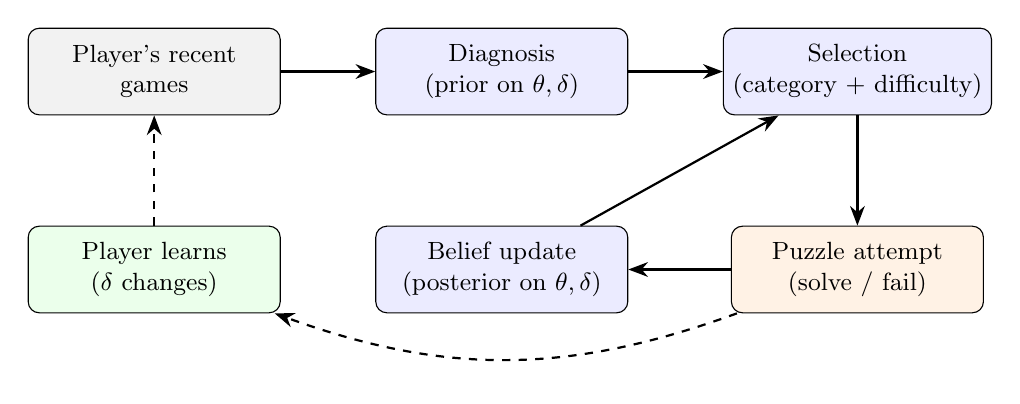
\begin{tikzpicture}[
  box/.style={draw, rounded corners, align=center, minimum width=3.2cm, minimum height=1.1cm, font=\small},
  arr/.style={-{Stealth[length=2.5mm]}, thick}]
  \node[box, fill=gray!10] (games) {Player's recent\\games};
  \node[box, fill=blue!8, right=1.2cm of games] (diag) {Diagnosis\\(prior on $\theta,\delta$)};
  \node[box, fill=blue!8, right=1.2cm of diag] (select) {Selection\\(category $+$ difficulty)};
  \node[box, fill=orange!10, below=1.4cm of select] (attempt) {Puzzle attempt\\(solve / fail)};
  \node[box, fill=blue!8, below=1.4cm of diag] (update) {Belief update\\(posterior on $\theta,\delta$)};
  \node[box, fill=green!8, below=1.4cm of games] (learn) {Player learns\\($\delta$ changes)};
  \draw[arr] (games) -- (diag);
  \draw[arr] (diag) -- (select);
  \draw[arr] (select) -- (attempt);
  \draw[arr] (attempt) -- (update);
  \draw[arr] (update) -- (select);
  \draw[arr, dashed] (attempt) to[bend left=20] (learn);
  \draw[arr, dashed] (learn) -- (games);
\end{tikzpicture}
\caption{The player--puzzle--learning loop. Solid arrows are the system's own inference; dashed arrows
are the change in the player that the system must track.}\label{fig:loop}
\end{figure}

\section{Requirements and Design Goals}

\paragraph{Functional requirements.}
\begin{enumerate}[label=FR\arabic*]
  \item Fetch a player's public games and profile from Chess.com without authentication.
  \item Analyse every move with Stockfish; grade errors and record critical positions (opportunities)
        with their tactical category.
  \item Build a weakness profile and priors for the recommender.
  \item Mine puzzles with a unique solution from the player's own games.
  \item Serve puzzles adaptively, choosing category and difficulty, and update after every attempt.
  \item Log each attempt with the serving policy, the selection probability and the pre-outcome
        prediction, so that the system can be evaluated later.
\end{enumerate}

\paragraph{Non-functional requirements and design goals.}
\begin{itemize}
  \item \textbf{Reproducibility.} Engine analysis is limited by node count, not time, so the same game
        always gives the same result. Simulations use fixed seeds and common random numbers.
  \item \textbf{Testability.} The whole test suite runs offline, with no engine or network (231 tests).
  \item \textbf{Graceful degradation.} If Stockfish is missing, or a category has no puzzle in range,
        the system falls back instead of failing.
  \item \textbf{Privacy.} Research data is pseudonymised and only aggregates are published.
  \item \textbf{Honest evaluation.} Every numeric claim can be regenerated from a result file by a
        script.
\end{itemize}

\section{High-Level System Architecture}

Figure~\ref{fig:arch} shows the components and data flow.

\begin{figure}[H]
\centering
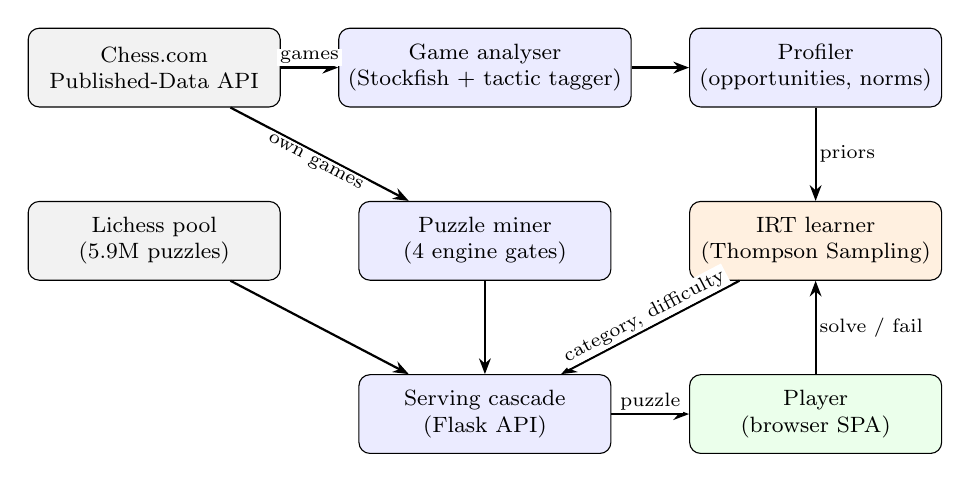
\begin{tikzpicture}[
  comp/.style={draw, rounded corners, align=center, minimum width=3.2cm, minimum height=1.0cm, font=\footnotesize},
  arr/.style={-{Stealth[length=2mm]}, thick},
  lab/.style={font=\scriptsize, fill=white, inner sep=1pt}]
  % three columns (x = 0, 4.2, 8.4) and three rows (y = 0, -2.2, -4.4)
  \node[comp, fill=gray!10]   (cc)    at (0,0)      {Chess.com\\Published-Data API};
  \node[comp, fill=blue!8]    (an)    at (4.2,0)    {Game analyser\\(Stockfish + tactic tagger)};
  \node[comp, fill=blue!8]    (prof)  at (8.4,0)    {Profiler\\(opportunities, norms)};
  \node[comp, fill=gray!10]   (pool)  at (0,-2.2)   {Lichess pool\\(5.9M puzzles)};
  \node[comp, fill=blue!8]    (mine)  at (4.2,-2.2) {Puzzle miner\\(4 engine gates)};
  \node[comp, fill=orange!12] (irt)   at (8.4,-2.2) {IRT learner\\(Thompson Sampling)};
  \node[comp, fill=blue!8]    (serve) at (4.2,-4.4) {Serving cascade\\(Flask API)};
  \node[comp, fill=green!8]   (ui)    at (8.4,-4.4) {Player\\(browser SPA)};
  \draw[arr] (cc) -- node[lab, above]{games} (an);
  \draw[arr] (an) -- (prof);
  \draw[arr] (cc) -- node[lab, sloped, below]{own games} (mine);
  \draw[arr] (prof) -- node[lab, right]{priors} (irt);
  \draw[arr] (mine) -- (serve);
  \draw[arr] (pool) -- (serve);
  \draw[arr] (irt) -- node[lab, sloped, above]{category, difficulty} (serve);
  \draw[arr] (serve) -- node[lab, above]{puzzle} (ui);
  \draw[arr] (ui) -- node[lab, right]{solve / fail} (irt);
\end{tikzpicture}
\caption{System architecture. The IRT learner decides the category and difficulty of the next puzzle,
and the serving cascade finds an unseen matching puzzle. Every attempt updates the learner and is
logged with the serving policy, the selection probability and the pre-outcome
prediction.}\label{fig:arch}
\end{figure}

The \textbf{game analyser} evaluates every player move after the opening with Stockfish. It grades
the move by the loss of win probability it causes, and records \emph{opportunities}, meaning
positions where the best move beats the runner-up by at least 10 percentage points of win
probability. The \textbf{tactic tagger} labels the engine's best line with one of the 23 categories.
The \textbf{profiler} turns found and missed opportunities into per-category estimates, shrunk
towards population norms. The \textbf{IRT learner} maintains a Gaussian posterior over $\theta_u$ and
the 23 offsets $\delta_{u,k}$. It chooses a category by Thompson Sampling, and a target difficulty
that gives a predicted 65\% solve rate. The \textbf{serving cascade} finds an unseen puzzle in that
category and rating window. It prefers puzzles mined from the player's own games, and widens its
constraints one at a time when nothing matches. The \textbf{miner} extracts puzzles from the player's
own losses through four verification gates.

\section{Chapter Summary}

The problem is formalised as sequential decision-making under uncertainty, based on a Rasch-type
model with a category-specific ability offset. The system implements that model online, with
evidence from games as a prior and puzzle attempts as the main source of information. The
requirements stress reproducibility, offline testability and evaluation that can be checked, and
these shape the methodology in the next chapter.

\chapter{Methodology}\label{ch:method}

\section{Data Sources and Preprocessing}\label{sec:data}

\paragraph{Lichess puzzle database.} The open Lichess puzzle export~\cite{lichessdb} (CC0) contains
roughly six million puzzles. Each has a starting position (FEN), a solution in UCI notation, a
Glicko-2 rating with its deviation, a popularity score, a play count and theme tags. A streaming ETL
reads the 1.1\,GB CSV in chunks of one million rows. It removes duplicates, puzzles with rating
deviation above 150, unplayed puzzles and empty solutions, leaving \textbf{5,877,641 puzzles}. At
server start a second quality gate filters on popularity, play count and solution length, and a
bounded, category-stratified sample of 199,998 puzzles is kept in memory.

A \emph{motif-priority} rule maps Lichess's roughly fifty raw theme tags onto the project's 23
categories. Tags arrive in alphabetical order, so an earlier ``first tag wins'' rule let the phase tag
\emph{endgame} outrank real motifs. It mislabelled about 198,000 of 305,000 puzzles then marked
Endgame (Section~\ref{sec:challenges}). The fixed rule resolves ties by specificity: forced mate,
then concrete motif, then generic attack, then endgame type.

\paragraph{Chess.com games.} Games are fetched from the public Chess.com Published-Data
API~\cite{chesscomapi}. The fetcher walks the player's monthly archives from newest to oldest,
caches every response on disk, and waits between requests as the platform's guidance asks.

\paragraph{Application logs.} Every puzzle attempt in the deployed application is stored with its
timestamp, puzzle, category, rating and outcome. For attempts made since the upgrade it also records
the serving policy, the selection probability and the model's prediction before the outcome. At the
time of writing the logs contain 123 attempts by five players.

\paragraph{Research cohort.} Five app users are far too few to evaluate the player models, so a
cohort was collected from the public API. It contains \textbf{300 players}, 60 in each of five rating
bands (below 1000, 1000--1399, 1400--1799, 1800--2199, 2200 and above). Players had to be active (a
rated rapid or blitz game within the last year) and experienced (at least 100 games in that time
control). Candidate players came from three sources:
\begin{enumerate}
  \item \emph{snowball sampling}: opponents of already-collected players whose game rating fell in a
        band that still needed players;
  \item Chess.com's titled-player lists;
  \item random members of the country player lists.
\end{enumerate}
Country lists alone are dominated by beginners, so the upper bands would never fill without the first
two sources. The cost is that the cohort is not a uniform random sample of Chess.com
(Section~\ref{sec:validity}). For each player the newest 60 rated standard-chess games were
analysed, about 18,000 games in total. Players are stored under a salted SHA-256 pseudonym.

\section{Player Modelling and Style Classification}\label{sec:player-model}

\subsection{Move grading by win probability}

Each player move after the first eight half-moves is analysed with Stockfish at a fixed budget of
75,000 nodes, using MultiPV~2 (the best move and the runner-up). Centipawn scores $c$ (from the side
to move) are mapped to win percentages with the curve Lichess uses~\cite{lichessaccuracy}:

\begin{equation}
  W(c) \;=\; 50 + 50\left(\frac{2}{1+e^{-0.00368208\,c}} - 1\right).
\end{equation}

\noindent The loss caused by a move is $L = W(c_{\text{best}}) - W(c_{\text{played}}) \geq 0$. Moves
are graded as inaccuracies, mistakes or blunders at $L\geq 5$, $10$ and $15$ percentage points. Win
probability is used instead of raw centipawns because the same centipawn loss means very different
things in different positions. A 300-centipawn loss is a blunder at $+50$ but only an inaccuracy at
$+900$, where the game is already decided.

\subsection{Opportunities: measuring weakness with a denominator}

A position is \emph{critical}, an opportunity, when the best move beats the runner-up by at least 10
win-percentage points. A simple recapture of a piece the opponent has just taken is excluded, because
it is usually the only move without being a tactic. Each opportunity is labelled with the tactic of
the engine's best line (Section~\ref{sec:features}), and is recorded as a \emph{hit} if the player's
move lost fewer than 5 points.

Counting errors alone is misleading. A player who meets many fork positions will make more fork
errors even if they convert most of them. The quantity of interest is the hit rate per category,
$\text{hits}_k / \text{opportunities}_k$.

\subsection{Weighting and hierarchical shrinkage}

Games are ranked from newest to oldest. Game $g$ receives weight $w_g = 0.5^{\text{rank}/25} \cdot
\tau(\text{time class})$, with $\tau = 0.5$ for bullet, $0.85$ for blitz and $1$ for rapid. Recent
games count more; bullet games count less, because time pressure rather than tactical knowledge drives
many bullet errors.

Each category's weighted hit count is then shrunk towards an \emph{expected} rate, the rate that is
typical for category $k$ at this player's overall level:

\begin{equation}
  e_{u,k} = \sigma\!\bigl(\operatorname{logit}(h_u) + o_k\bigr), \qquad
  \hat r_{u,k} = \frac{\text{hits}_{u,k} + S\,e_{u,k}}{n_{u,k} + S},
\end{equation}

\noindent Here $h_u$ is the player's overall hit rate. The population offset $o_k =
\operatorname{logit}(h_k) - \operatorname{logit}(h)$ says how much harder or easier category $k$ is
for everyone. It is fitted on the research cohort from 23,796 opportunities, for example $+1.71$ for
pawn endgames and $-0.74$ for sacrifices. The strength $S$ is chosen by cross-validation over
players, and was 128--256 in every fold. The original profiler, which shrank towards $h_u$ alone,
misread ``this motif is hard for everyone'' as ``this player is weak at it''.

\subsection{Rating-group classification (Objective O1)}\label{sec:rating-method}

For each cohort player, 18 features are computed from their analysed games, describing \emph{how}
they play:
\begin{itemize}
  \item mean and median win-percentage loss, and mean centipawn loss;
  \item blunders, mistakes and inaccuracies per game;
  \item the share of errors in the opening, middlegame and endgame;
  \item opportunities per game, and the overall hit rate;
  \item hit rates for tactical, mating, endgame and quiet-move groups;
  \item mean game length, win rate, and the share of blitz games.
\end{itemize}
The PGN rating headers of both players are \emph{excluded}, because they would leak the label. The
classifiers are a multinomial logistic regression on standardised features and a random
forest~\cite{breiman2001random}, both from scikit-learn~\cite{pedregosa2011scikit}. They are
evaluated with stratified 5-fold cross-validation over players, repeated ten times, and a
500-shuffle permutation test.

\begin{honest}[Honest status: style]
The portfolio's style classification (positional, attacking, defensive) was not built as a learned
model. A rule-based archetype heuristic (\code{style\_profile.py}) assigns labels such as ``Tactical
Attacker'' from termination patterns and sacrifice rates, but it has no ground truth and was not
validated. Unsupervised style discovery in the manner of Jayasekara~\cite{jayasekara2018classification}
is left as future work.
\end{honest}

\section{Puzzle Representation and Feature Design}\label{sec:features}

A puzzle is a FEN position before the opponent's last move, followed by a solution line in UCI
notation, which alternates the player's moves and forced replies. Its category comes from the
motif-priority rule for Lichess puzzles, or from the tactic tagger for mined puzzles and game
opportunities.

\paragraph{The tactic tagger.} The original labeller looked at the first move only and used a few
geometric tests. It was measured to agree with Lichess themes on only 31\% of puzzles
(Section~\ref{sec:labeller-results}). The replacement tags the \emph{whole line}:
\begin{itemize}
  \item A line the engine scores as a forced mate is a \emph{Mating Pattern}, whatever its first move
        looks like.
  \item A \emph{fork} requires the moved piece to attack at least two targets. Each target must be
        the king, worth more than the attacker, or undefended. The forking piece must not simply be
        lost to a cheaper capture, and a king only counts as a capturer if the square is undefended.
  \item \emph{Pin} and \emph{skewer} come from ray geometry. Walking outward from a line piece, let
        $P_1$ be the first enemy piece and $P_2$ the second. If $P_2$ is the king or worth more than
        $P_1$, it is a pin. If $P_1$ is the king or worth more than $P_2$, it is a skewer.
  \item A \emph{discovered attack} is recorded when another of the player's line pieces newly attacks
        a valuable or undefended target.
  \item \emph{Endgame types} come from the material left on the board (for example, only rooks and
        pawns means a rook endgame), not from which piece moved.
  \item Only the first two player moves may contribute combination motifs; later moves may add only
        promotion or mate. Incidental pins and pawn captures deep in a continuation were the main
        source of false positives.
\end{itemize}
Five categories are never emitted: Attraction, Interference, Clearance, Zugzwang and X-Ray. They need
deeper reasoning about the line, and emitting nothing is preferable to guessing.

\section{PuzzleNet: a Neural Model of Tactic and Difficulty}\label{sec:puzzlenet}

Two measured weaknesses motivate a learned model, and both are documented in
Chapter~\ref{ch:results}. First, every weakness estimate in the system inherits the tactic labeller's
errors, and the hand-written tagger of Section~\ref{sec:features} agrees with Lichess themes on only
58\% of held-out puzzles ($\kappa = 0.52$), while never emitting five of the categories at all. The
label-quality experiment (E3) shows that perfect labels would raise early targeting well beyond what
the tagger achieves, so labelling is a real bottleneck rather than a cosmetic one. Second, a mined
puzzle's difficulty is a closed-form guess from the size of the player's error and the length of the
solution; it is uncalibrated, carries no uncertainty, and 67.5\% of all real attempts were on mined
puzzles.

Both are supervised learning problems for which a large, free, labelled dataset already exists: the
5.88 million Lichess puzzles, each carrying theme tags and a Glicko-2 rating with its own deviation.
\textbf{PuzzleNet} is a single multi-task network trained on that dataset. It reads a position and the
line that follows it, and predicts the line's tactical category, its Lichess theme tags, and how
difficult it is, with an uncertainty attached to that difficulty.

\subsection{Task definition}

Let $s_0$ be a position with the \emph{solver} to move and $L = (m_1, r_1, m_2, r_2, \dots)$ the
principal line from it, alternating solver moves $m_i$ and replies $r_i$. The same pair $(s_0, L)$
occurs in all three places the system needs a label: a Lichess puzzle (the solution line), a critical
position in an analysed game (Stockfish's principal variation), and a mined puzzle (the forced
continuation built by the miner). The network estimates three things:

\begin{align}
  P(\text{category} = c \mid s_0, L), \quad c \in \{1,\dots,24\}, \\
  P(\text{theme}_j = 1 \mid s_0, L), \quad j \in \{1,\dots,66\}, \\
  b \mid s_0, L \;\sim\; \mathcal{N}\!\left(\mu(s_0, L),\; \sigma^2(s_0, L)\right),
\end{align}

\noindent where $b$ is the puzzle's difficulty on the Lichess rating scale. The theme head is an
auxiliary task: theme tags are a richer description of the same line, and predicting them gives the
shared trunk more to learn from than a single label per puzzle.

\subsection{Input representation}

The input is a fixed vector of 3{,}329 features. Its design follows two principles: give the network
the raw board, and also give it the relations a tactician would look for, so that it need not
rediscover the rules of attack and defence from piece positions alone. Whether the second part earns
its place is an ablation, not an assumption (Section~\ref{sec:ablations}).

Everything is encoded \emph{from the solver's point of view}. When Black is to move, squares are
mirrored ($a1 \leftrightarrow a8$) and colours swapped, so that the solver's pieces always occupy the
first six planes and the solver's pawns always advance up the board. A position and its
colour-mirrored twin therefore produce the identical vector, which halves what the network must learn
and is checked by a unit test on real puzzles.

\begin{itemize}
  \item \textbf{Boards} (2{,}304 bits). Piece-square planes ($12 \times 64$) for three positions:
        before the key move, after it, and after the solver's second move.
  \item \textbf{Moves} (864 bits). Six move blocks: the opponent move that created the position, then
        $m_1, r_1, m_2, r_2, m_3$. Each block holds the from-square, the to-square, the moving piece,
        the captured piece, and flags for check, promotion, under-promotion, castling and en passant.
  \item \textbf{Tactical relations} (90 bits). For each of the first three solver moves: which enemy
        piece types the moved piece attacks, whether it attacks two or more valuable targets, whether
        it is left en prise or defended, discovered and double checks, pins it creates and the types
        of pinned pieces, a piece lined up behind an attacked king, queen or rook, whether the move is
        quiet, a retreat, or captures a defender, and whether the position after it is checkmate.
  \item \textbf{Replies} (6 bits) and \textbf{position facts} (43 bits): forced replies and recaptures;
        hanging pieces on both sides; whether the key move is the only check or the only capture;
        castling rights; the material signature of an endgame; a boxed-in king; the number of solver
        moves in the line; and the mate verdict.
  \item \textbf{Continuous features} (27). Material by piece type and the balance before and after the
        line, the number of legal moves, captures and checks available, pressure on the squares around
        the enemy king and its escape squares, and the number of replies the opponent had.
\end{itemize}

No engine evaluation enters the encoding, so all 5.88M puzzles can be encoded in under an hour on a
laptop, and a position can be encoded during game analysis in about three milliseconds. The one
exception is an optional mate flag, which lets game analysis pass Stockfish's mate verdict for a line
that was cut off before the mate appears.

\subsection{Architecture}

A shared trunk of two fully connected ReLU layers ($3{,}329 \to 512 \to 256$) feeds three linear
heads: a 24-way softmax for the category, 66 independent sigmoids for the themes, and two outputs
$(\mu, s)$ for the difficulty, where $\sigma^2 = e^{s}$. The network has 1.86M parameters. Sharing a
trunk across the three tasks is classical multi-task learning~\cite{caruana1997multitask}: the
representation that says \emph{which} tactic a line contains is largely the representation that says
how hard it is to find.

\subsection{Loss: a noise-aware heteroscedastic objective}

For a batch, with $y_c$ the category, $\mathbf{y}_t$ the theme indicators and $y_b$ the observed
rating (standardised), the loss is

\begin{equation}\label{eq:puzzlenet-loss}
  \mathcal{L} = \underbrace{-\log p_{y_c}}_{\text{category}}
  \;+\; \lambda_t \sum_{j} \mathrm{BCE}\bigl(\sigma(z_{t,j}), y_{t,j}\bigr)
  \;+\; \lambda_r \, \underbrace{\mathrm{sg}\!\left(v^{\beta}\right)}_{\text{$\beta$-NLL weight}}
  \cdot \tfrac{1}{2}\left[\log v + \frac{(y_b - \mu)^2}{v}\right],
\end{equation}

\begin{equation}\label{eq:puzzlenet-var}
  v \;=\; \underbrace{e^{s}}_{\text{content uncertainty}} \;+\; \underbrace{\rho^2}_{\text{known rating noise}} .
\end{equation}

\noindent Two choices in this objective matter for how the model is used later.

\paragraph{Known label noise.} A Lichess rating is not the truth about a puzzle; it is a Glicko-2
estimate that comes with its own deviation $\rho$ (a median of 79 rating points, but far larger for
rarely played puzzles). Equation~\eqref{eq:puzzlenet-var} adds that known measurement variance to the
model's own, so that a noisy label pulls the fit less than a precise one, and so that $e^{s}$ is left
to represent only what the content itself leaves uncertain: how hard this puzzle is, given what is on
the board. That is exactly the quantity the recommender needs for a mined puzzle, which has no
Lichess rating at all, and it is why the variance head is not decoration. Section~\ref{sec:integration-irt}
shows where it enters the Bayesian update.

\paragraph{$\beta$-NLL.} Training a Gaussian likelihood with a learned variance has a known failure
mode: the network can reduce the loss on hard examples by inflating their variance, which in turn
scales down their gradient for the mean, so the hardest examples end up teaching the mean the least.
Seitzer et al.~\cite{seitzer2022pitfalls} correct this by weighting each example's loss by a
stop-gradient copy of $v^\beta$. With $\beta = 1$ the mean receives exactly the plain squared-error
gradient; with $\beta = 0$ the plain likelihood is recovered. This work uses the recommended
$\beta = 0.5$, and both extremes are run as ablations.

\subsection{Optimisation and calibration}

The network, its gradients and its optimiser are written from first principles in
NumPy~\cite{harris2020array}; no deep learning framework is used. Two reasons: the deployed
application keeps no heavy dependency and answers in about a millisecond on a CPU, and every step of
the learning algorithm stays visible and testable. Each hand-derived gradient is checked against
central finite differences in the test suite, for every head and for the linear, single-task and
multi-task configurations.

Training uses AdamW~\cite{loshchilov2019decoupled} (decoupled weight decay on weight matrices only),
gradient-norm clipping, and a learning rate that warms up linearly and then decays on a cosine
schedule~\cite{loshchilov2017sgdr}, with batches of 2{,}048 and He initialisation for the ReLU
layers~\cite{he2015delving}. Model selection keeps the checkpoint with the best validation score.

Raw network outputs are then calibrated on the validation split by fitting two scalars: a softmax
temperature $T$ for the category head~\cite{guo2017calibration}, and a variance scale $c$ such that
$v = c\,e^{s} + \rho^2$ for the difficulty head, in the spirit of post-hoc recalibration for
regression~\cite{kuleshov2018accurate}. Both are one-dimensional optimisations of the validation
likelihood, and both are reported before and after in Chapter~\ref{ch:results}.

\subsection{Data, splits and a fair comparison}

Puzzles are split by a hash of their identifier: 2\% validation, 3\% test, the rest for training.
One further set is carved out first. The rule-based tagger was scored in
Section~\ref{sec:labeller-results} on a held-out sample of 30{,}000 uniformly drawn puzzles plus up to
2{,}000 per category; those 59{,}668 puzzles are \emph{excluded from training and model selection
entirely}, so that both labellers can be scored on exactly the same puzzles, neither having seen them.
The tagger's development sample is not excluded, because the stratified draw takes up to 2{,}000 of
each category and the rarest category has only about 2{,}100 puzzles in total; holding out both
samples would have left the network almost no examples of them.

\subsection{Where the network enters the system}\label{sec:integration-irt}

\begin{enumerate}
  \item \textbf{Labelling critical positions.} Game analysis labels the engine's principal variation
        with PuzzleNet instead of the rule-based tagger. Because game analysis sees an engine line
        rather than a puzzle solution, this shift of input distribution is measured separately
        (Section~\ref{sec:nn-deployment}), and the number of plies the network is shown is chosen from
        that measurement.
  \item \textbf{Rating mined puzzles.} A mined puzzle takes $\mu$ as its rating and $\sigma$ as its
        rating deviation, replacing the closed-form heuristic and the blanket deviation of 300 points.
        The deviation is floored at 75 points, the deviation of a well-played Lichess puzzle: a puzzle
        nobody has ever attempted cannot be known more precisely than that, and the model was
        calibrated on Lichess puzzles rather than on puzzles mined from a player's own games.
  \item \textbf{Feeding the Bayesian recommender.} That per-puzzle deviation is the term $v_b$ in the
        IRT update of Section~\ref{sec:rl-setup}: $\kappa = (1 + 3 v_b / \pi^2)^{-1/2}$ scales how far
        one attempt may move a player's ability and category offsets. An uncertain difficulty estimate
        now moves the player's model less, instead of every mined puzzle being treated as equally
        uncertain.
\end{enumerate}

Every one of these paths falls back to the previous behaviour when no model file is installed or when
\code{PUZZLENET=off} is set, and the rule-based tagger remains available through \code{LABELLER=rules}.
The application therefore still runs, unchanged, without the network.

\subsection{What it is compared against}

The category head is compared with the rule-based tagger on the held-out harness, with paired tests on
the same puzzles (McNemar's exact test~\cite{mcnemar1947note} on per-puzzle correctness and bootstrap
intervals for the differences in $\kappa$ and macro recall). The difficulty head is compared with the
miner's formula, with a constant, with a least-squares fit on line length and the mate verdict, and
with gradient-boosted trees~\cite{ke2017lightgbm} trained on the hand-built features alone. Ablations
trained on a common one-million-puzzle subset isolate the contributions of depth, of the hand-built
features, of the raw board, of multi-task learning and of the $\beta$-NLL exponent, and a
learning-curve sweep from 30{,}000 to 5.5 million puzzles shows how much the data volume matters.
Finally, the labels are carried downstream: into the label-quality simulation, into the 300-player
cohort, and into the prequential replay of the real solve logs.


\section{Generative Model Design}\label{sec:generation}

\begin{honest}[Honest status: no generative model was built]
The portfolio planned a generative model fine-tuned with reinforcement learning to create new puzzles,
optimised for uniqueness and counter-intuitiveness, following Feng et al.~\cite{feng2025generating}.
This was \textbf{not implemented}. That approach needs millions of training puzzles, a neural
generator, and an RL loop in which every candidate is scored by engine search, a compute budget far
beyond an individual MSc project. The implemented alternative, \emph{engine-verified mining} from the
player's own games, meets the legality and uniqueness requirements of Objective O2 by construction.
It does not produce puzzles that are new to the world, and it does not optimise
counter-intuitiveness.
\end{honest}

\paragraph{Engine-verified mining.} For each move the player made, four gates must all pass
(the constants are listed in Appendix~\ref{app:constants}):
\begin{enumerate}
  \item \emph{Detection}: the player's move is at least 150 centipawns worse than the engine's best.
  \item \emph{Clarity}: the best move beats the runner-up by at least 100 centipawns, which rules out
        a second solution.
  \item \emph{Forcing}: each opponent reply in the continuation is at least 80 centipawns better than
        its alternative.
  \item \emph{Verification}: a depth-18 re-analysis confirms the solution.
\end{enumerate}
An earlier miner used heuristics without an engine and produced about 40\% false positives; it was
removed. Accepted puzzles are labelled by the tactic tagger. Their difficulty is estimated by a
closed-form heuristic from the size of the error and the length of the solution. That heuristic is
uncalibrated, and replacing it is a stated item of future work (Section~\ref{sec:future}).

\section{Reinforcement Learning Setup}\label{sec:rl-setup}

The recommendation problem is formulated as a multi-armed bandit: one arm per category, with Bernoulli
rewards (solved or not). This is reinforcement learning in its simplest setting, a single state with
repeated actions~\cite{sutton2018reinforcement}. It is \emph{not} deep reinforcement learning: there is
no neural policy, no value network and no multi-step planning.

\subsection{Beta--Bernoulli Thompson Sampling (original policy)}

Each category $k$ has a posterior $\text{Beta}(\alpha_k,\beta_k)$ over its solve rate. The update is
exact by conjugacy: $\alpha_k \leftarrow \alpha_k + y$ and $\beta_k \leftarrow \beta_k + 1 - y$. The
selection rule draws $\tilde\theta_k \sim \text{Beta}(\alpha_k,\beta_k)$ for every category and serves
$\arg\min_k \tilde\theta_k$. This is the \emph{minimum}, not the maximum of standard
TS~\cite{russo2018tutorial}, because the goal is to practise weaknesses. Priors come from the profile,
with a pseudo-count that grows with the evidence: $C_k = \min(10, n_k+2)$, $\alpha_k = 1 + \hat
r_k C_k$, $\beta_k = 1 + (1-\hat r_k) C_k$. An optional discount $\gamma$ pulls every arm back towards
its prior after each update, as in the discounted TS of Raj and Kalyani~\cite{raj2017taming}. It is
switched off by default, for reasons given in Section~\ref{sec:ablations}.

This policy has a structural flaw. Failing a 2200-rated puzzle and failing a 1000-rated one change
$\beta_k$ by the same amount, so categories that happen to be served harder puzzles look weaker.

\subsection{Difficulty-aware IRT learner with Thompson Sampling (new default)}

The new policy keeps a Gaussian posterior $\mathcal{N}(\mathbf{m}, \mathbf{S})$ over $\mathbf{w} =
(\theta, \delta_1,\dots,\delta_{23})$, with full $24\times24$ covariance, for the model in
Equation~\eqref{eq:rasch}. For an attempt in category $k$ at difficulty $b$, whose own uncertainty is
$v_b$, let $\mathbf{x} = \mathbf{e}_\theta + \mathbf{e}_k$. One online Laplace (extended-Kalman) step
gives:

\begin{align}
  \kappa &= \bigl(1 + 3 v_b / \pi^2\bigr)^{-1/2}, \qquad
  p = \sigma\!\bigl(\kappa(\mathbf{x}^\top\mathbf{m} - b)\bigr), \qquad
  h = \kappa^2 p(1-p), \\
  \mathbf{S}' &= \mathbf{S} - \frac{h\,\mathbf{S}\mathbf{x}\mathbf{x}^\top\mathbf{S}}{1 + h\,\mathbf{x}^\top\mathbf{S}\mathbf{x}}, \\
  \mathbf{m}' &= \mathbf{m} + \frac{\kappa\,(y - p)\,\mathbf{S}\mathbf{x}}{1 + h\,\mathbf{x}^\top\mathbf{S}\mathbf{x}}.
\end{align}

\noindent With one parameter this is term for term the Glicko update: $\kappa$ is Glicko's $g(\phi_j)$,
$p$ is $E$ and $h$ is $1/v$. A unit test checks the equivalence to $10^{-9}$ against the Glicko-2
implementation, which itself reproduces Glickman's published worked example (1464.06 / 151.52 /
0.05999)~\cite{glickman2012example}. Because the covariance is full, evidence from a failed puzzle is
split between ``weak overall'' ($\theta$) and ``weak at this motif'' ($\delta_k$). Before each update
the learner adds random-walk drift, $\mathbf{S} \leftarrow \mathbf{S} + \operatorname{diag}(0.02^2,
0.04^2,\dots)$, so that it can follow a player who is improving.

\paragraph{Selection.} Draw $\tilde{\mathbf{w}} \sim \mathcal{N}(\mathbf{m},\mathbf{S})$ and serve
$\arg\min_k \tilde\delta_k$. This is Thompson Sampling on the difficulty-adjusted category offsets.

\paragraph{Priors.} $\delta_k$ is centred on $\operatorname{logit}(\hat r_{u,k}) -
\operatorname{logit}(e_{u,k})$, the player's deviation from what is typical. The information credited
to game evidence is $0.5 \cdot \tfrac{n}{n+S} \cdot n\,\hat r(1-\hat r)$. The factor $0.5$ reflects
that finding a move in a game and solving a flagged puzzle are related but different tasks. The factor
$n/(n+S)$ keeps the prior wide when pooling dominates, so that puzzle attempts can still move it.

\section{Adaptive Curriculum / Recommendation Strategy}

After choosing a category $k$, the learner sets a target difficulty at which the predicted solve
probability equals $p^\star = 0.65$:

\begin{equation}
  b^\star = m_\theta + m_{\delta_k} - \operatorname{logit}(p^\star), \qquad
  r^\star = 1500 + 173.7178\, b^\star ,
\end{equation}

\noindent and the serving window is $r^\star \pm 150$. The choice of $p^\star$ follows the
zone-of-proximal-development argument~\cite{vygotsky1978mind}: hard enough to demand effort, easy enough
to succeed usually. Its sensitivity is tested in Section~\ref{sec:ablations}.

The \emph{serving cascade} looks for an unseen puzzle in this order:
\begin{enumerate}
  \item the player's own mined puzzles in category $k$ and the rating window;
  \item any unseen mined puzzle, 40\% of the time;
  \item the Lichess pool, category $k$, within the window;
  \item the same, with the window widened by $\pm 200$;
  \item any category within the window;
  \item any category at any rating;
  \item a repeat, flagged as such.
\end{enumerate}
Each served puzzle records the policy, the Monte Carlo selection probability of the chosen category,
and the prediction made before the outcome. These make calibration checks and off-policy evaluation
possible later, as in Nie et al.~\cite{nie2026discovering}.

\section{Evaluation Metrics}\label{sec:metrics}

\begin{table}[H]
\centering
\small
\caption{Metrics used in Chapter~\ref{ch:results}.}\label{tab:metrics}
\begin{tabularx}{\linewidth}{p{0.27\linewidth}Y}
\toprule
\textbf{Metric} & \textbf{Definition} \\
\midrule
Strict / lenient agreement & Tagger label equals the Lichess primary category / is among any category the puzzle's themes map to. \\
Cohen's $\kappa$ & Chance-corrected agreement, interpreted on the Landis and Koch scale~\cite{landis1977measurement}. \\
Targeting rate & Share of served categories that are among the player's true three weakest. \\
Regret & $\sum_t (\delta_{k_t} - \min_k \delta_k)$ in logits (Equation~\eqref{eq:regret}). \\
Frustration / productive zone & Share of served puzzles with true $P(\text{solve})<0.30$ / in $[0.50, 0.85]$. \\
Learning gain & Mean improvement of $\delta$ in the initially weak categories (simulation only). \\
Log loss, Brier, AUC & Proper scoring of predicted probabilities on held-out outcomes. \\
Prequential log loss & Each attempt is predicted before the model learns from it~\cite{dawid1984present}. \\
Accuracy, macro-F1 & Rating-band classification; also accuracy within one band. \\
Split-half reliability & Correlation of a player's category deviations between odd and even games. \\
\bottomrule
\end{tabularx}
\end{table}

\noindent\textbf{Statistics.} Policy comparisons use common random numbers, so that every policy meets
the same simulated player for a given seed. They are analysed as paired differences, with paired
$t$-tests, Wilcoxon signed-rank tests, Cohen's $d_z$, bootstrap 95\% confidence intervals and Holm
correction~\cite{holm1979simple} across the policies compared.

\chapter{Implementation}\label{ch:implementation}

\section{Technology Stack and Tools}

\begin{table}[H]
\centering
\small
\caption{Technology stack.}\label{tab:stack}
\begin{tabularx}{\linewidth}{p{0.3\linewidth}Y}
\toprule
\textbf{Layer} & \textbf{Technology} \\
\midrule
Language & Python 3.13 \\
Board logic, PGN, UCI & python-chess~\cite{pythonchess} \\
Engine & Stockfish 18~\cite{stockfish} (bundled Windows binary) \\
Numerics and machine learning & NumPy, SciPy, scikit-learn~\cite{pedregosa2011scikit} \\
Data & pandas~\cite{mckinney2010data}, PyArrow (Parquet, read one row group at a time) \\
Web application & Flask with a vanilla-JavaScript single-page front end, served from one origin \\
Persistence & JSON files per user (no database) \\
Testing & pytest, 231 tests, fully offline \\
Figures and reports & Matplotlib; HTML reports printed to PDF \\
Version control & Git, feature branch \code{feature/adaptive-engine} \\
\bottomrule
\end{tabularx}
\end{table}

\section{System Modules}

\begin{table}[H]
\centering
\small
\caption{Main modules.}\label{tab:modules}
\begin{tabularx}{\linewidth}{p{0.38\linewidth}Y}
\toprule
\textbf{Module} & \textbf{Responsibility} \\
\midrule
\code{src/api/chess\_com\_fetcher.py} & Chess.com client with disk cache and rate limiting \\
\code{src/data/puzzle\_loader.py} & Lichess loading, cleaning, the 23-category taxonomy and motif priority \\
\code{src/classifier/stockfish\_analyzer.py} & Deterministic MultiPV analysis, win-probability grading, opportunities \\
\code{src/puzzles/tactic\_tagger.py} & Line-level tactic tagging \\
\code{src/classifier/player\_profiler.py} & Profile, hierarchical shrinkage with population norms, priors \\
\code{src/data/category\_norms.json} & Population category offsets and shrinkage strength (aggregates only) \\
\code{src/recommender/irt\_model.py} & Difficulty-aware IRT learner with Thompson Sampling (default policy) \\
\code{src/recommender/bandit.py} & Beta--Bernoulli Thompson bandit (the original policy, kept for comparison) \\
\code{src/analysis/difficulty\_fitter.py} & Glicko-2 fitter (frozen-pool mode, prequential hook) \\
\code{src/classifier/ml\_weakness\_model.py} & Random-forest weakness model (optional, trained on simulated players) \\
\code{src/puzzles/generator.py} & Four-gate puzzle miner \\
\code{src/evaluation/simulation.py} & Simulation environment: synthetic players, policies, episodes \\
\code{web/backend/app.py} & Flask API: analysis, sessions, serving cascade, logging \\
\code{scripts/research/*} & Labeller validation, simulation study, cohort collection and analysis, evaluations, report \\
\bottomrule
\end{tabularx}
\end{table}

\subsection{The neural module}\label{sec:nn-implementation}

PuzzleNet adds one package and one training pipeline; Table~\ref{tab:nn-modules} lists them.

\begin{table}[H]
\centering
\small
\caption{Neural components.}\label{tab:nn-modules}
\begin{tabularx}{\linewidth}{p{0.36\linewidth}Y}
\toprule
\textbf{Module} & \textbf{Responsibility} \\
\midrule
\code{src/neural/encoding.py} & Position and line to a 3{,}329-feature vector; colour-canonical by construction \\
\code{src/neural/network.py} & The network, its loss, hand-derived backpropagation, AdamW, save and load \\
\code{src/neural/dataset.py} & Targets, splits, feature subsets, and a bounded-memory block loader \\
\code{src/neural/metrics.py} & Calibration fitting, category, theme and rating metrics \\
\code{src/neural/predictor.py} & The trained model as the analyzer, miner and app use it \\
\code{src/puzzles/labeller.py} & Chooses the neural or the rule-based labeller \\
\code{scripts/neural/build\_dataset.py} & Encodes all 5.88M puzzles in parallel \\
\code{scripts/neural/train\_puzzlenet.py} & One training run; \code{run\_experiments.py} runs all of them \\
\code{scripts/neural/evaluate\_puzzlenet.py} & Harness, test split, baselines and ablations \\
\code{scripts/neural/engine\_pv\_check.py} & Deployment condition: labelling Stockfish lines \\
\code{scripts/neural/relabel\_cohort.py} & Relabels the 300-player cohort's critical positions \\
\bottomrule
\end{tabularx}
\end{table}

\paragraph{Data pipeline.} Encoding 5.88M puzzles is a pure-Python workload (python-chess move
generation and attack maps), so it runs in twelve worker processes. Each puzzle becomes 3{,}302 bits,
packed into 413 bytes, plus 27 half-precision values: 2.4\,GB for the whole database, small enough to
keep on disk and read as needed. The whole build takes 48 minutes on the development laptop and is
verified row by row against direct encoding.

\paragraph{Bounded memory.} The development machine has 16\,GB of RAM, of which about 4\,GB were free
in practice. Two designs had to be changed for that. The dataset builder originally held every FEN in
the parent process and wrote through a memory map, which grew the working set to several gigabytes; it
was rewritten to stream record batches from the Parquet file with a bounded number of chunks in
flight, writing results with ordinary file writes. Training reads the feature file through a memory
map, and the loader (\code{BlockLoader}) draws mini-batches by reading one contiguous block of rows at
a time and shuffling within it, shuffling the block order between epochs. Rows are stored in puzzle-id
order, which is random with respect to content, so block shuffling mixes the data well while touching
only a small part of the 2.4\,GB file at once. Training never exceeds about 2\,GB.

\paragraph{Correctness.} The backward pass is hand-derived, so it is tested rather than trusted: for
every head and for the linear, single-task and multi-task configurations, each analytic gradient is
compared with a central finite difference of an independently written reference loss, in double
precision. The encoder is tested on real puzzles for colour symmetry (a position and its mirrored twin
give identical vectors) and for individual features: a knight fork sets the double-attack bit, a
back-rank mate sets the mate bits, a bishop move that creates an absolute pin sets the pin bits, and
so on. In total the neural code adds 56 tests to the suite.

\paragraph{Deployment.} The trained model is exported in half precision to
\code{src/data/models/puzzlenet.npz}, 3.6\,MB, and loaded once per process. Inference is three matrix
products and takes about a millisecond per position, on top of the three milliseconds needed to encode
it; game analysis already spends far longer than that on the engine search for the same position. The
application keeps no deep learning dependency: NumPy, which it already used, is enough. If the model
file is absent, if it was trained with a different encoding version, or if \code{PUZZLENET=off} is
set, every call site falls back to the previous rule-based behaviour, and the test suite runs with the
network disabled by default so that it tests that fallback path.


\section{Integration and Deployment Setup}

The whole application is served by one Flask process on port 5000: the API and the static front end
from the same origin. At start-up it streams the Parquet pool one row group at a time, never holding
all six million rows in memory, and applies the quality gate. Game analysis runs in a background
thread, and the browser polls for progress. The policy is chosen with environment variables:
\code{RECOMMENDER} (\code{irt} by default, or \code{beta}), \code{BANDIT\_DISCOUNT}, and
\code{WEAKNESS\_MODEL}. Both recommendation models are updated on every attempt, whichever one served
the puzzle, so switching policy never starts cold. A player who trained before the IRT learner
existed has a posterior rebuilt by replaying their stored history.

The research pipeline runs separately and reproducibly:
\begin{itemize}
  \item cohort collection (resumable, rate-limited);
  \item cohort analysis in worker processes;
  \item the evaluation scripts, which write JSON results;
  \item a report builder that reads only those JSON files, so that no number in a report is typed by
        hand.
\end{itemize}
Research data is kept in a git-ignored directory and stored under pseudonyms. Only aggregate results
are committed.

\section{Implementation Challenges and Solutions}\label{sec:challenges}

Several defects were found during the project by re-reading the code against its own documentation.
They are listed because some of them silently invalidated earlier behaviour, which matters for
interpreting anything measured before they were fixed.

\begin{table}[H]
\centering
\small
\caption{Defects found and how they were fixed.}\label{tab:defects}
\begin{tabularx}{\linewidth}{p{0.3\linewidth}Yp{0.25\linewidth}}
\toprule
\textbf{Defect} & \textbf{Consequence} & \textbf{Fix} \\
\midrule
Stockfish located with \code{shutil.which} only & The bundled engine was never found; every profile silently fell back to a crude heuristic & Use the project's resolver, which checks the bundled path \\
\code{multipv=1} returned a list & Every move analysis raised \code{TypeError}; hidden by the defect above & Drop the argument; found by a live smoke test \\
``First tag wins'' theme mapping & About 198k of 305k ``Endgame'' puzzles mislabelled & Motif-priority resolution, re-applied at load time \\
Accuracy formula fed centipawns & Lichess's accuracy formula takes win-\% loss, so a typical player showed about 15\% accuracy & Pass win-\% loss~\cite{lichessaccuracy} \\
Substring colour detection & ``bob'' against ``bobby\_99'' was assigned the wrong colour & Exact username match first \\
Priors truncated with \code{int()} & Fractional priors lost & Floats end to end \\
Time-limited search & The same game could give different errors on another run & Node-limited, deterministic search \\
Recaptures counted as opportunities & Hit rates inflated by trivial moves & Recapture filter \\
Country-list sampling & Cohort dominated by beginners & Snowball and titled-player sampling \\
Parallel pool crash on Windows & 14 processes $\times$ 16 BLAS threads oversubscribed the CPU & One BLAS thread per worker \\
Evaluation runtime & $O(n^2)$ recomputation (more than 10 minutes) & Statistics computed once per fold (1.7 minutes) \\
\bottomrule
\end{tabularx}
\end{table}

Two lessons stand out. First, \emph{``the tests pass'' and ``it works against a real engine'' are
different claims.} The offline test suite deliberately never calls Stockfish, so the
\code{multipv} defect was invisible to it; only a live run exposed it. Second, \emph{hypotheses about
performance should be measured before they are fixed.} A plausible diagnosis, that Python's global
interpreter lock limited the analysis thread pool, was refuted by a head-to-head benchmark: 127\,s
with threads against 129\,s with processes, with identical output. The design kept threads.

\chapter{Experiments and Results}\label{ch:results}

\section{Experimental Design and Baselines}

Table~\ref{tab:experiments} lists the experiments. The recommendation policies are compared with five
baselines:
\begin{itemize}
  \item \textbf{Random}: a uniform choice of category;
  \item \textbf{Round-robin}: cycling through all categories;
  \item \textbf{Static profile}: rotating through the three categories that look weakest from game
        history;
  \item \textbf{Greedy}: always the lowest posterior mean, with no exploration;
  \item \textbf{Oracle}: knows the player's true current $\delta$ and gives an upper bound.
\end{itemize}
The two adaptive policies are the original \textbf{Beta-TS} (with the Elo $\pm 300$ band) and the new
\textbf{IRT-TS}.

\begin{table}[H]
\centering
\small
\caption{Experiments and the research questions they address.}\label{tab:experiments}
\begin{tabularx}{\linewidth}{p{0.27\linewidth}Yp{0.1\linewidth}}
\toprule
\textbf{Experiment} & \textbf{Data and design} & \textbf{RQ} \\
\midrule
Tactic-label validation & 30,000 uniform and 48,000 stratified Lichess puzzles; development and held-out seeds & RQ3 \\
Puzzle-quality evaluation & 30 mined puzzles, five automatic criteria at depth 18 & RQ3 \\
Rating-group classification & 300 real players, 5 bands, CV over players, permutation test & RQ1 \\
Weakness diagnosis & 300 real players, temporal hold-out, 11,973 test opportunities & RQ2 \\
Prequential calibration & 123 real attempts by 5 app users & RQ4 \\
Simulation E1 & Pre-registered protocol, 200 runs & RQ5 \\
Simulation E2--E7 & Semi-synthetic players, 200 paired runs per condition & RQ4, RQ5 \\
\bottomrule
\end{tabularx}
\end{table}

\section{Offline Evaluation of Puzzle Quality and Difficulty}

\subsection{Quality of mined puzzles}

The five-criterion evaluator re-analyses each mined puzzle with Stockfish at depth 18.
Table~\ref{tab:quality} reports it for the 30 puzzles mined for one app user rated 1050.

\begin{table}[H]
\centering
\small
\caption{Automatic quality of 30 mined puzzles (one player).}\label{tab:quality}
\begin{tabular}{lr}
\toprule
\textbf{Criterion} & \textbf{Result} \\
\midrule
Engine agrees the intended move is best & 30 / 30 (100\%) \\
No dual solution (gap $\geq 50$ cp) & 27 / 30 (90\%) \\
Strong clarity (PV1 $-$ PV2 $\geq 150$ cp) & 11 / 30 (37\%) \\
Solution depth $\geq 3$ ply & 30 / 30 (100\%) \\
Trivial free capture & 0 / 30 \\
Difficulty within $\pm 300$ of player rating & 25 / 30 (83\%) \\
Mean composite score & 0.869 \\
\bottomrule
\end{tabular}
\end{table}

The mining gates produce puzzles that are sound: engine agreement and depth are perfect, and 90\% have
no second solution. Only 37\% reach the stricter clarity threshold, so many puzzles have a plausible
second-best move. This is a single player's sample and indicative only.

\subsection{Tactic-label validation}\label{sec:labeller-results}

\begin{table}[H]
\centering
\small
\caption{Tactic labeller against Lichess themes, held-out sample (seed 11).}\label{tab:labeller}
\begin{tabular}{lrr}
\toprule
\textbf{Metric} & \textbf{Original (first move)} & \textbf{New tagger (whole line)} \\
\midrule
Strict agreement & 31.2\% & \textbf{58.4\%} \\
Lenient agreement & 37.4\% & \textbf{60.9\%} \\
Cohen's $\kappa$ & 0.23 & \textbf{0.52} \\
Macro recall (stratified) & 14.4\% & \textbf{32.0\%} \\
Macro precision (uniform) & 30.3\% & \textbf{53.7\%} \\
Categories never emitted & 8 & 5 \\
\bottomrule
\end{tabular}
\end{table}

On the development sample (seed 7) the new tagger scores 57.6\% ($\kappa=0.51$), almost the same as on
the held-out sample. The improvement is therefore not an artefact of tuning. The largest per-class
gains are for Mating Pattern (recall 0.46 to 0.998), Skewer (0.12 to 0.76), Discovered Attack (0.08
to 0.69) and Promotion (0.08 to 0.64). The original's ``Fork'' was a catch-all, with recall 0.82 and
precision only 0.25; the new tagger's Fork precision is 0.61. Agreement of $\kappa=0.52$ is
``moderate''~\cite{landis1977measurement}. The tagger is much better than before, but still far from
perfect, and its errors spread across related motifs (Figure~\ref{fig:labeller}).

\begin{figure}[H]
\centering
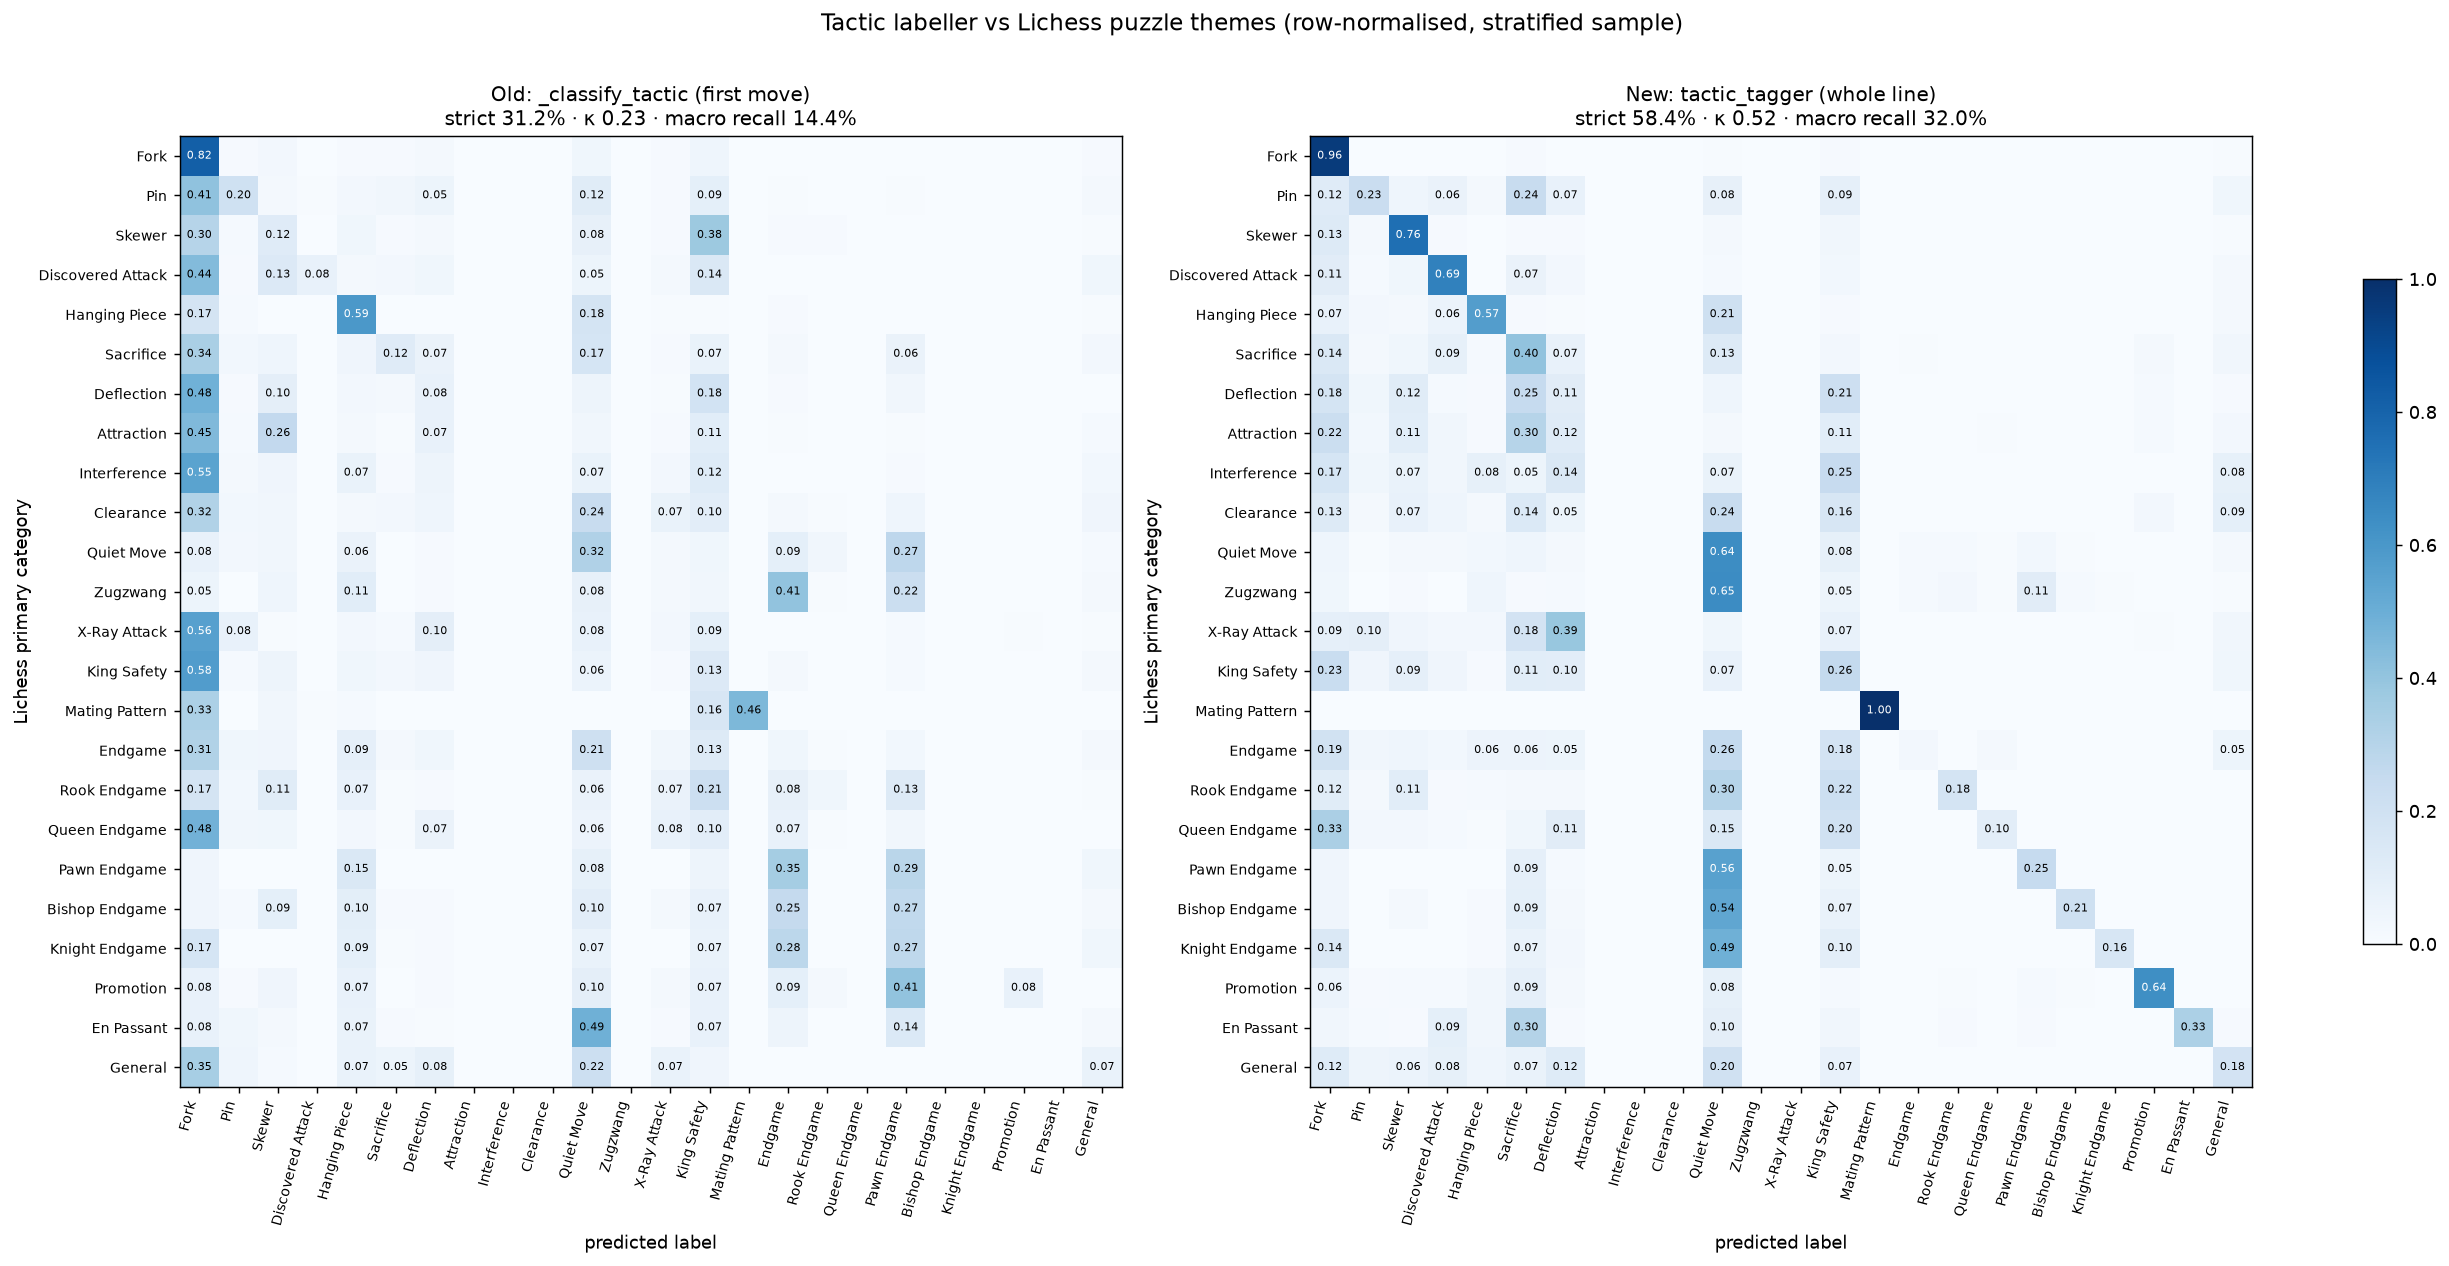
\includegraphics[width=\linewidth]{figures/labeller_confusion_heldout.png}
\caption{Row-normalised confusion matrices of the original and new taggers against Lichess themes
(held-out sample).}\label{fig:labeller}
\end{figure}

\subsection{Difficulty calibration on real solve logs}

Every model replays the 123 real attempts in time order and predicts each one before learning from it.
Players solved \textbf{84.6\%} of attempts; 67.5\% of the puzzles were mined from their own games.

\begin{table}[H]
\centering
\small
\caption{Prequential evaluation on real attempts ($n=123$, 5 players).}\label{tab:prequential}
\begin{tabular}{lrrrrr}
\toprule
\textbf{Model} & \textbf{Log loss} & \textbf{Brier} & \textbf{AUC} & \textbf{Mean pred.} & $\boldsymbol{\Delta}$\textbf{LL vs Elo [95\% CI]} \\
\midrule
Base rate (running mean) & 0.451 & 0.139 & 0.51 & 0.77 & $-0.758$ [$-1.013$, $-0.513$] \\
Static Elo (original) & 1.208 & 0.374 & 0.54 & 0.45 & reference \\
Glicko-2, symmetric & 0.640 & 0.212 & 0.58 & 0.69 & $-0.569$ [$-0.759$, $-0.375$] \\
Glicko-2, pool frozen & 0.714 & 0.242 & 0.46 & 0.69 & $-0.495$ [$-0.692$, $-0.296$] \\
IRT, $\theta$ only & 0.652 & 0.222 & 0.49 & 0.70 & $-0.556$ [$-0.764$, $-0.348$] \\
IRT, per category & 0.599 & 0.202 & 0.54 & 0.71 & $-0.609$ [$-0.812$, $-0.406$] \\
\bottomrule
\end{tabular}
\end{table}

\begin{finding}
The original assumption, comparing a player's Chess.com rating with a puzzle's Lichess rating (the
basis of the Elo $\pm300$ band), is badly miscalibrated. It predicts a 45\% solve rate where players
achieved 84.6\%, and its log loss (1.21) is worse than a coin flip (0.69). Every learned model corrects
this, with confidence intervals that exclude zero, and the per-category IRT is the best of them. With
only 123 events, however, no model yet discriminates \emph{which} puzzles will be solved (AUC close to
0.5), so a constant base rate is still the best calibrated. This limit is set by the amount of data.
\end{finding}

\begin{figure}[H]
\centering
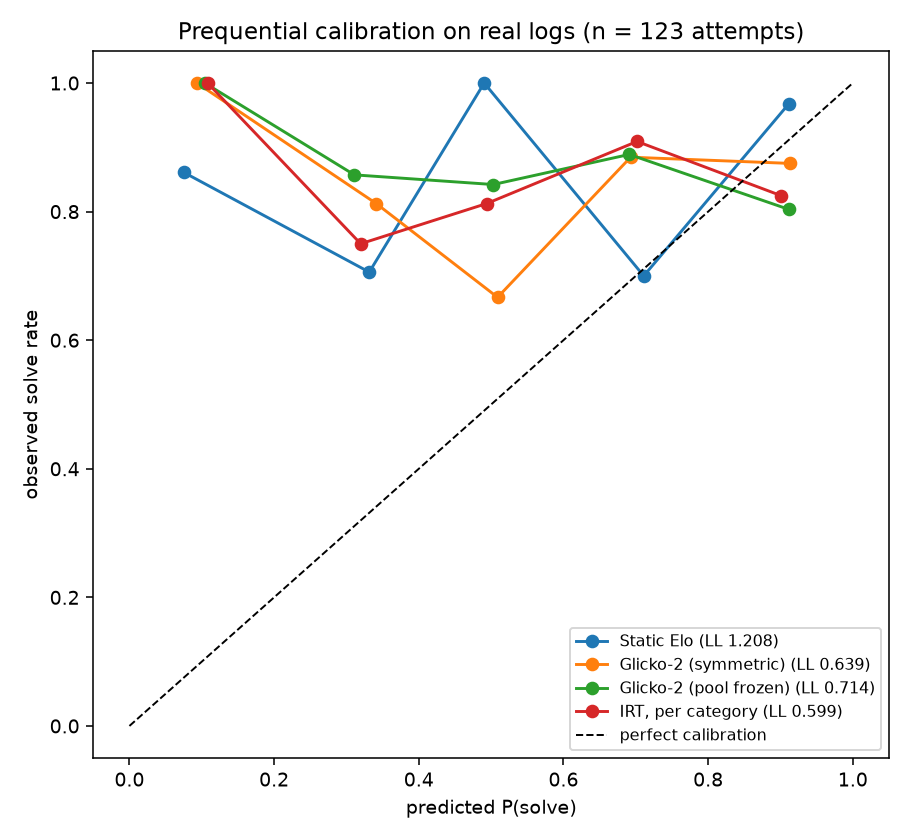
\includegraphics[width=0.62\linewidth]{figures/difficulty_calibration.png}
\caption{Calibration of the prequential predictions on the real logs.}\label{fig:calibration}
\end{figure}

\section{The Neural Tactic and Difficulty Model}\label{sec:nn-results}

PuzzleNet was trained on the 5{,}526{,}626 puzzles of the training split for three epochs (8{,}097
updates of 2{,}048 puzzles), which took 42 minutes on the development laptop's CPU. The 59{,}668
puzzles of the held-out labeller harness were excluded from training and from model selection, so the
comparison below is on exactly the puzzles the rule-based tagger was scored on in
Section~\ref{sec:labeller-results}, with neither labeller having seen them.

\subsection{Tactic labelling}\label{sec:nn-labelling}

\begin{table}[H]
\centering
\small
\caption{Labeller agreement with Lichess themes on the held-out harness (seed 11). Uniform sample
$n = 30{,}000$; stratified sample $n = 48{,}000$. The rule-based row reproduces
Section~\ref{sec:labeller-results} exactly, which confirms that both labellers see the same
puzzles.}\label{tab:nn-harness}
\begin{tabularx}{\linewidth}{Xccccc}
\toprule
\textbf{Labeller} & \textbf{Strict} & \textbf{Lenient} & \textbf{$\kappa$} & \textbf{Macro recall} & \textbf{Macro precision} \\
\midrule
Rule-based tagger & 58.4\% & 60.9\% & 0.516 & 0.320 & 0.537 \\
\textbf{PuzzleNet} & \textbf{92.6\%} & \textbf{93.1\%} & \textbf{0.913} & \textbf{0.859} & \textbf{0.877} \\
\bottomrule
\end{tabularx}
\end{table}

\begin{finding}[The labeller stops being the bottleneck]
Agreement rises from 58.4\% to 92.6\% and $\kappa$ from 0.52 to 0.91, which moves the labeller from
``moderate'' to ``almost perfect'' on the Landis and Koch scale~\cite{landis1977measurement}. Because
both labellers ran on the same puzzles, the comparison is paired: PuzzleNet is right on 10{,}671
puzzles where the rules are wrong, and wrong on 424 where the rules are right (McNemar's exact test,
$p < 10^{-300}$). Bootstrap 95\% intervals for the differences are $+33.6$ to $+34.7$ points of
agreement, $+0.391$ to $+0.403$ of $\kappa$, and $+0.536$ to $+0.543$ of macro recall.
\end{finding}

\begin{figure}[H]
\centering
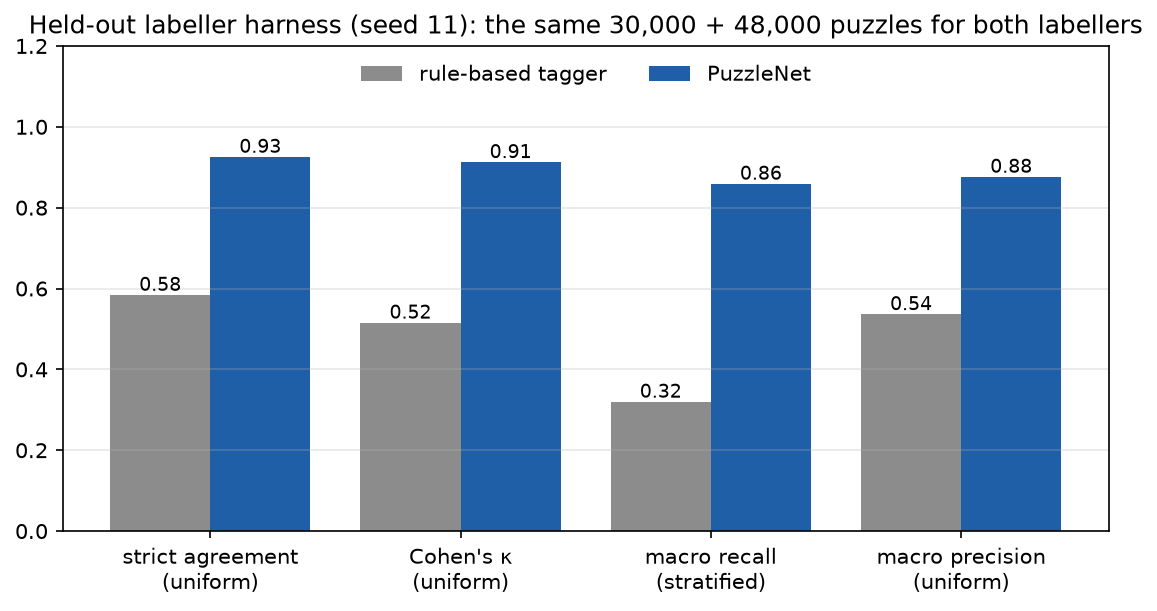
\includegraphics[width=\linewidth]{figures/nn_harness_comparison.png}
\caption{Both labellers on the held-out harness. The samples are the same puzzles that Section~\ref{sec:labeller-results} used, and neither labeller saw them during development.}\label{fig:nn-harness}
\end{figure}

The gain is largest where the rules were weakest. Macro recall nearly triples, because the tagger's
failures were structural rather than a matter of tuning: five of the 24 categories (Attraction,
Interference, Clearance, Zugzwang and X-Ray Attack) could never be emitted at all, since no
hand-written test existed for them, so their recall was zero by construction. PuzzleNet emits every
category, and learns the five missing ones from examples alone. Its remaining confusions are mostly
with the residual class \emph{General}, in both directions (for example 82 pins called General and 75
Generals called Pin): those are puzzles whose Lichess tags name no motif, where the boundary is
genuinely soft.

\begin{table}[H]
\centering
\small
\caption{Per-category recall on the stratified harness sample (2{,}000 puzzles per category where the
database has that many). The five categories in the upper block have no hand-written test at all, so
the rule-based tagger can never emit them; PuzzleNet learns them from examples.}\label{tab:nn-perclass}
\begin{tabularx}{\linewidth}{Xcccc}
\toprule
& \multicolumn{2}{c}{\textbf{Recall}} & \multicolumn{2}{c}{\textbf{Precision}} \\
\cmidrule(lr){2-3}\cmidrule(lr){4-5}
\textbf{Category} & Rules & PuzzleNet & Rules & PuzzleNet \\
\midrule
Attraction        & 0.000 & 0.869 & --- & 0.840 \\
Interference      & 0.000 & 0.714 & --- & 0.815 \\
Clearance         & 0.000 & 0.413 & --- & 0.590 \\
Zugzwang          & 0.000 & 0.618 & --- & 0.774 \\
X-Ray Attack      & 0.000 & 0.648 & --- & 0.909 \\
\midrule
En Passant        & 0.331 & 0.929 & 0.78 & 0.895 \\
Pin               & 0.227 & 0.798 & 0.43 & 0.833 \\
General           & 0.180 & 0.925 & 0.61 & 0.889 \\
Fork              & \textbf{0.956} & 0.934 & 0.61 & 0.922 \\
Mating Pattern    & 0.999 & 1.000 & 1.00 & 1.000 \\
\bottomrule
\end{tabularx}
\end{table}

Fork is the one category where the rule-based tagger has the higher recall (0.956 against 0.934), and
it shows what a rule tuned for recall costs elsewhere: its fork precision is 0.61, against 0.92 for the
network, so two of every five positions it called a fork were something else, and that misdirected
evidence went into a player's fork arm. Fourteen of the 24 categories now reach a recall of 0.9 or
better. The weakest are Clearance (0.41), Zugzwang (0.62) and X-Ray Attack (0.65) --- the motifs that
depend on what does \emph{not} happen in a line, or on long-range geometry, which a
position-and-move encoding captures least well. Lenient agreement, which accepts any category the
puzzle's own themes map to, rises from 60.9\% to 95.1\%.

\subsection{Difficulty prediction}\label{sec:nn-difficulty}

On the 174{,}754 test puzzles, the difficulty head reaches an RMSE of 268 rating points and a mean
absolute error of 205, against a rating standard deviation of 550: it explains $R^2 = 0.76$ of the
variance, with a rank correlation of $\rho = 0.88$ with the Lichess rating. The predictions are
essentially unbiased overall (mean error $-0.8$ points), but they regress to the mean at the extremes,
as any squared-error regression does: $+114$ points on puzzles rated below 1000 and $-390$ on those
above 2500.

\begin{table}[H]
\centering
\small
\caption{Difficulty prediction on the 174{,}754 test puzzles. Every baseline gets a constant
predictive standard deviation fitted on the validation split, so that the likelihoods are comparable.
The miner's formula needs an engine evaluation drop, which a Lichess puzzle does not have, so it is
evaluated with that term fixed at the median of the puzzles actually mined from users' games
(312 centipawns), which makes it a function of solution length.}\label{tab:nn-rating-baselines}
\begin{tabularx}{\linewidth}{Xcccc}
\toprule
\textbf{Difficulty model} & \textbf{RMSE} & \textbf{MAE} & \textbf{$R^2$} & \textbf{$\rho$} \\
\midrule
Constant (training mean)                          & 550 & 459 & 0.00 & --- \\
The miner's formula (what PuzzleNet replaces)     & 496 & 390 & 0.19 & 0.55 \\
Least squares on line length $\times$ mate verdict & 433 & 351 & 0.38 & 0.61 \\
Gradient-boosted trees on the hand-built features & 306 & 239 & 0.69 & 0.84 \\
\textbf{PuzzleNet}                                & \textbf{268} & \textbf{205} & \textbf{0.76} & \textbf{0.88} \\
\bottomrule
\end{tabularx}
\end{table}

The formula the system used until now explains 19\% of the variance in puzzle difficulty; the network
explains 76\%. The comparison that matters more, though, is with the gradient-boosted trees, because
they see the same hand-built tactical features and are a strong classical model on tabular data: the
network is 38 rating points better on RMSE, and on the category task it beats them by $\kappa = 0.91$
against $0.79$ with a calibration error of 0.003 against 0.123. Whatever the network is adding, it is
not only the feature engineering.

What matters more for the recommender is that the uncertainty is honest. The predictive intervals cover
what they claim to cover: 50.1\%, 81.2\% and 95.3\% of the test puzzles fall inside the nominal 50\%,
80\% and 95\% intervals. The mean content uncertainty is 240 rating points, which is the number a
mined puzzle now carries into the Bayesian update in place of the blanket 300.

\begin{table}[H]
\centering
\small
\caption{The trained network on seven textbook positions built by hand for the unit tests, none of
them from the puzzle database. $p$ is the calibrated probability of the chosen category; the rating is
the predicted difficulty with its content uncertainty.}\label{tab:nn-examples}
\begin{tabularx}{\linewidth}{Xlccl}
\toprule
\textbf{Position} & \textbf{PuzzleNet} & \textbf{$p$} & \textbf{Rating} & \textbf{Rule tagger} \\
\midrule
Back-rank mate in 1            & Mating Pattern & 1.00 & $477 \pm 83$   & Mating Pattern \\
Knight forks king and rook     & Fork           & 0.72 & $1026 \pm 196$ & Fork \\
Bishop pins knight to the king & Pin            & 0.63 & $1201 \pm 282$ & Pin \\
Rook skewers king, wins queen  & Skewer         & 1.00 & $696 \pm 58$   & Skewer \\
Pawn promotes                  & Promotion      & 0.98 & $857 \pm 162$  & Promotion \\
En passant capture             & En Passant     & 1.00 & $1137 \pm 194$ & En Passant \\
Rook ladder, mate in 2         & Mating Pattern & 1.00 & $1339 \pm 155$ & Mating Pattern \\
\bottomrule
\end{tabularx}
\end{table}

Both labellers agree on all seven, which is the expected result: these are the clean cases the rules
were written for. The interesting column is the difficulty. The network has never seen these
positions, yet it rates the mate in one at 477 with a tight interval and the two-move rook ladder at
1339, and it is least sure about the pin ($\pm 282$), which is the position whose difficulty depends
most on what the defender can try next.

\begin{figure}[H]
\centering
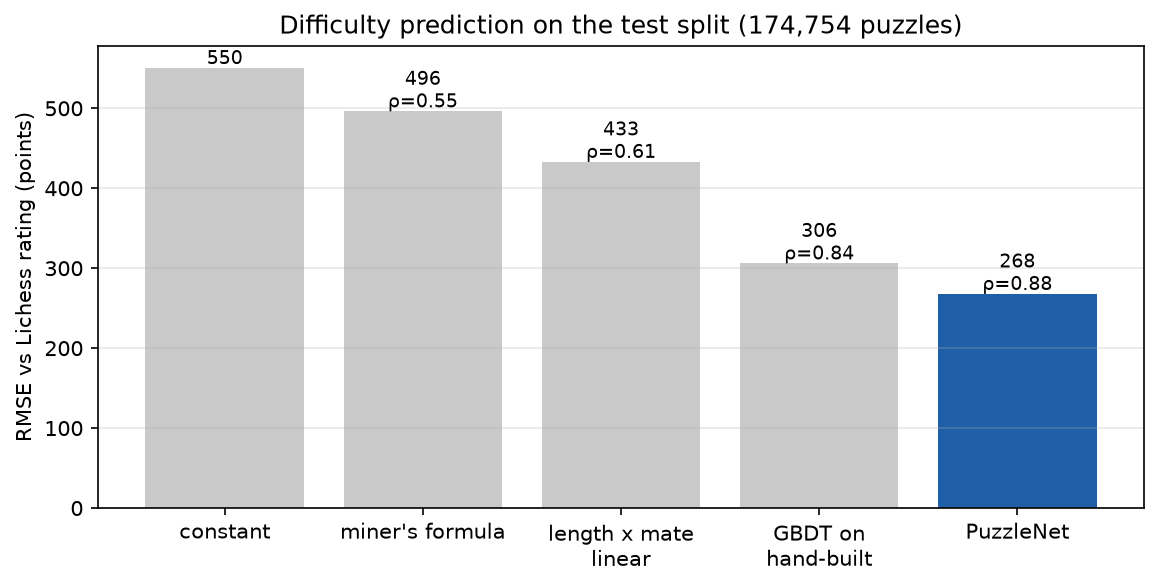
\includegraphics[width=\linewidth]{figures/nn_rating_baselines.png}
\caption{Difficulty prediction on the test split against the non-neural baselines: a constant, the miner's fixed formula, a least-squares fit on line length and the mate verdict, and gradient-boosted trees on the hand-built features. $\rho$ is the rank correlation with the Lichess rating.}\label{fig:nn-rating}
\end{figure}

\subsection{Themes and calibration}

The auxiliary theme head reaches a micro-averaged $F_1$ of 0.913 and a mean average precision of 0.817
over the 66 Lichess themes with enough positives to score. The category head is already well calibrated
before any correction (expected calibration error 0.0055) and essentially perfectly calibrated after
temperature scaling with $T = 1.08$ (0.0026). The variance scale fitted for the difficulty head is
1.05, that is, the learned variances needed almost no correction. Good calibration is not a
presentational detail here: the probabilities are consumed by the recommender, so a model that is
confidently wrong would corrupt a player's profile.

\subsection{Labelling engine lines, which is what the application actually does}\label{sec:nn-deployment}

Every number so far comes from puzzle solution lines. In the application the labeller sees something
else: Stockfish's principal variation from a critical position in a real game, cut to a fixed number
of plies. A puzzle solution stops when the tactic is complete; an engine line runs on into the won
position that follows. To measure that shift, 2{,}000 held-out harness puzzles were re-analysed with
the analyzer's own settings, and both labellers were scored on the engine line and on the solution
line of the same puzzles.

\begin{table}[H]
\centering
\small
\caption{Agreement with the Lichess category on 2{,}000 held-out puzzles, by the line the labeller is
shown. The engine's first move is the puzzle's first solution move in 99.3\% of these positions, so
the difference is about the line, not about the engine finding something else.}\label{tab:nn-engine}
\begin{tabularx}{\linewidth}{Xcc}
\toprule
\textbf{Line shown to the labeller} & \textbf{Strict agreement} & \textbf{$\kappa$} \\
\midrule
Rule-based tagger, puzzle solution        & 56.9\% & 0.504 \\
Rule-based tagger, engine line (7 plies)  & 55.5\% & 0.489 \\
\midrule
PuzzleNet, puzzle solution                & 91.9\% & 0.905 \\
PuzzleNet, engine line (1 ply)            & 66.4\% & 0.602 \\
PuzzleNet, engine line (3 plies)          & 80.3\% & 0.769 \\
\textbf{PuzzleNet, engine line (5 plies)} & \textbf{80.9\%} & \textbf{0.777} \\
PuzzleNet, engine line (7 plies)          & 76.5\% & 0.726 \\
\bottomrule
\end{tabularx}
\end{table}

\begin{honest}[Honest status: the network loses a third of its advantage in deployment]
PuzzleNet was trained on solution lines, so the engine line costs it a great deal: $\kappa$ falls from
0.91 to 0.78. The rule-based tagger barely moves (0.50 to 0.49), because it restricts which motifs may
be claimed at which depth and so ignores most of the continuation anyway. The deployed advantage is
therefore $\kappa = 0.78$ against $0.49$, not $0.91$ against $0.52$. It is still a large advantage,
and it is the honest one to quote for game analysis.
\end{honest}

The table also fixes a parameter. Agreement peaks when the network is shown five plies, and drops by
0.05 of $\kappa$ at seven, which is what the analyzer previously passed to the tagger. The deployed
system now gives the network the first five plies (\code{labeller.NEURAL\_PV\_PLIES}) and the
rule-based tagger the full line it was validated on. That is a measured choice, not a guess.

\subsection{What the network is actually learning: ablations}\label{sec:nn-ablations}

Every ablation trains on the same one-million-puzzle subset with the same schedule and is scored on
the same test split, so the rows differ only in what is named. The table is generated from
\code{eval/neural/puzzlenet\_evaluation.json} by \code{dissertation/build\_ablation\_table.py}, so it
cannot drift from the experiments.

\begin{table}[H]
\centering
\small
\caption{Ablations (1M training puzzles each) and the data-scaling sweep, all on the same test
split. $\kappa$ and macro-$F_1$ are the category head; RMSE is the difficulty head in rating points; a
dash means the model has no such head. Training times are not comparable across rows: the runs
shared a loaded laptop.}\label{tab:nn-ablations}
\begin{tabularx}{\linewidth}{Xcccc}
\toprule
\textbf{Variant} & \textbf{$\kappa$} & \textbf{Macro-$F_1$} & \textbf{RMSE} & \textbf{Train (s)} \\
\midrule
Reference: 512--256 trunk, all features, all heads & 0.867 & 0.774 & 285 & 516 \\
\midrule
No hidden layers (logistic / linear regression) & 0.743 & 0.610 & 326 & 294 \\
Raw boards and moves only & 0.741 & 0.645 & 313 & 505 \\
Hand-built relations only (no boards, no moves) & 0.830 & 0.708 & 305 & 74 \\
Wider trunk: 1024--512 & 0.878 & 0.797 & 280 & 4907 \\
\midrule
Category head alone (no multi-task) & 0.870 & 0.782 & --- & 486 \\
Difficulty head alone (no multi-task) & --- & --- & 280 & 468 \\
$\beta = 0$ (plain noise-aware likelihood) & 0.860 & 0.763 & 283 & 562 \\
$\beta = 1$ (squared-error gradient for the mean) & 0.868 & 0.777 & 289 & 250 \\
\midrule
30{,}000 training puzzles & 0.722 & 0.570 & 351 & 95 \\
100{,}000 & 0.780 & 0.654 & 333 & 127 \\
300{,}000 & 0.823 & 0.708 & 297 & 122 \\
1{,}000{,}000 & 0.867 & 0.774 & 285 & 516 \\
\textbf{5{,}526{,}626 (the production model)} & \textbf{0.914} & \textbf{0.861} & \textbf{268} & \textbf{2478} \\
\bottomrule
\end{tabularx}
\end{table}

\begin{finding}[Representation and data, not capacity]
The hand-built tactical relations carry most of the signal: on their own, with no boards and no move
blocks at all, they reach $\kappa = 0.830$ against $0.867$ for the full input. The raw boards and
moves on their own reach $0.741$. Each still adds something the other lacks --- the relations add
$0.126$ to the raw input, the raw input adds $0.037$ to the relations --- but a reader should not
conclude that the network has learned chess from squares. Depth matters about as much as the
relations: with no hidden layers, on the same features, $\kappa$ falls to $0.743$. Capacity is the
cheapest thing to buy and the least useful: four times the trunk buys $0.011$, while 5.5 times the
data buys $0.047$ and the curve has not flattened.
\end{finding}

\begin{figure}[H]
\centering
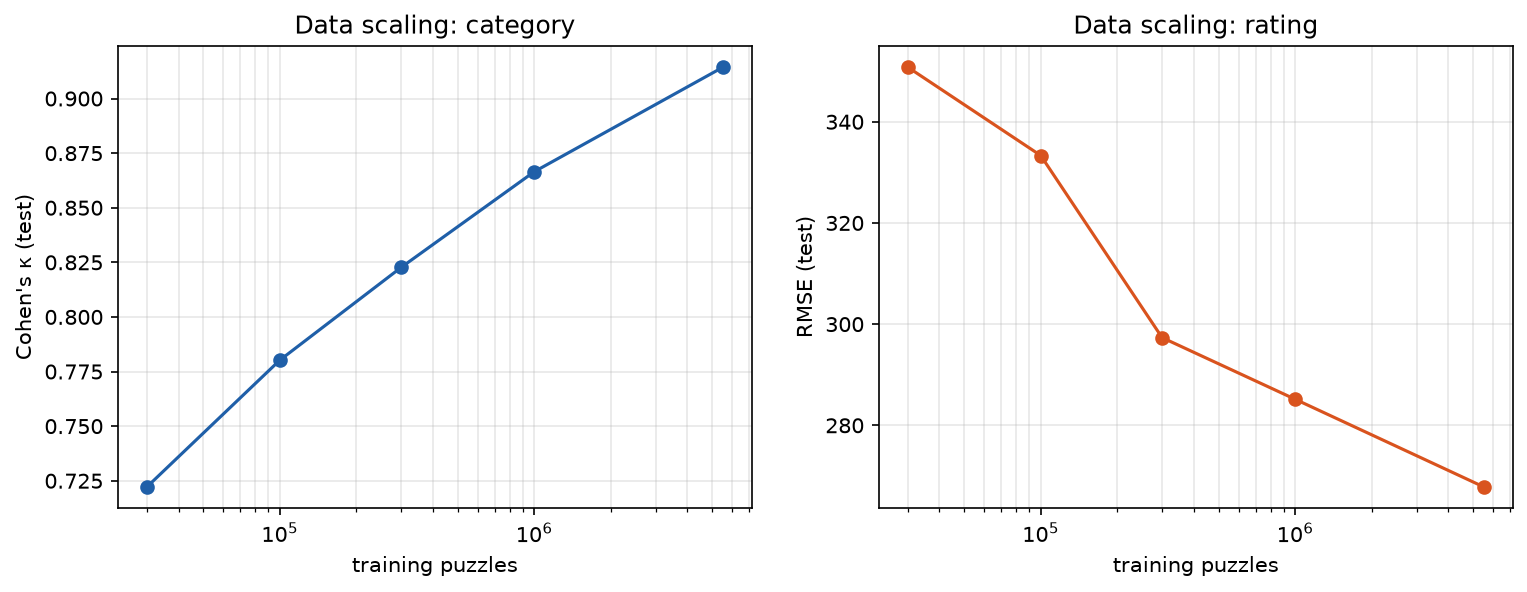
\includegraphics[width=\linewidth]{figures/nn_data_scaling.png}
\caption{Data scaling. Both heads keep improving to the full 5.5M puzzles; the curve has not flattened, so the model is limited by data rather than by capacity.}\label{fig:nn-scaling}
\end{figure}

Two results are negative and worth stating plainly. First, \textbf{multi-task learning does not help
either task here}: the category head alone reaches $\kappa = 0.870$ against $0.867$ when it shares a
trunk with themes and difficulty, and the difficulty head alone reaches RMSE 280 against 285. The
shared trunk costs a little on each task; what it buys is one model, one encoding pass and one file
instead of two, which is why the deployed model keeps it. Second, \textbf{the $\beta$-NLL correction
is not doing much work}. Plain noise-aware likelihood ($\beta = 0$) gives the best RMSE of the three
(283 against 285 at $\beta = 0.5$ and 289 at $\beta = 1$), and the differences are small either
way. The pathology that motivates
$\beta$-NLL~\cite{seitzer2022pitfalls} is that a learned variance can silence hard examples; here the
dominant part of the variance is the puzzle's \emph{known} rating deviation, and down-weighting a
noisily labelled puzzle is exactly the right thing to do, so the correction has little left to fix. On
another dataset without known label noise the argument for it would be stronger.


\subsection{Downstream: does better labelling help the recommender?}\label{sec:nn-downstream}

A labeller is only worth what it changes. Three downstream tests follow, one simulated and two on real
data, and they do not all point the same way.

\paragraph{Simulation: the label-quality bottleneck closes.} Experiment E3
(Section~\ref{sec:ablations}) measured how much early weak-category targeting depends on label
quality, by drawing each observed label from the labeller's measured $P(\text{predicted} \mid
\text{true})$. Rerunning it with PuzzleNet's confusion matrix, on the same 200 seeds so that every
comparison is paired:

\begin{table}[H]
\centering
\small
\caption{Weak-category targeting over the first 30 puzzles, by the source of the game evidence
(200 paired runs, $T = 60$).}\label{tab:nn-labelsim}
\begin{tabularx}{\linewidth}{Xcc}
\toprule
\textbf{Label source} & \textbf{Beta-TS} & \textbf{IRT-TS} \\
\midrule
No game evidence              & 0.148 & 0.151 \\
Rule-based tagger             & 0.189 & 0.226 \\
\textbf{PuzzleNet}            & \textbf{0.245} & \textbf{0.306} \\
Perfect labels                & 0.239 & 0.321 \\
\bottomrule
\end{tabularx}
\end{table}

\begin{finding}[PuzzleNet labels are statistically indistinguishable from perfect ones]
For the IRT policy, PuzzleNet beats the rule-based tagger by $+0.080$ targeting
(95\% CI $+0.055$ to $+0.105$, $p = 7 \times 10^{-10}$, $d_z = 0.46$), and the remaining gap to
\emph{perfect} labels is $+0.015$ and not significant ($p = 0.31$). It closes 84\% of the
rules-to-perfect gap for IRT-TS and all of it for Beta-TS. Cumulative regret falls from 62.6 to 55.3,
against 53.2 with perfect labels. The bottleneck identified in E3 is, in simulation, gone.
\end{finding}

\begin{figure}[H]
\centering
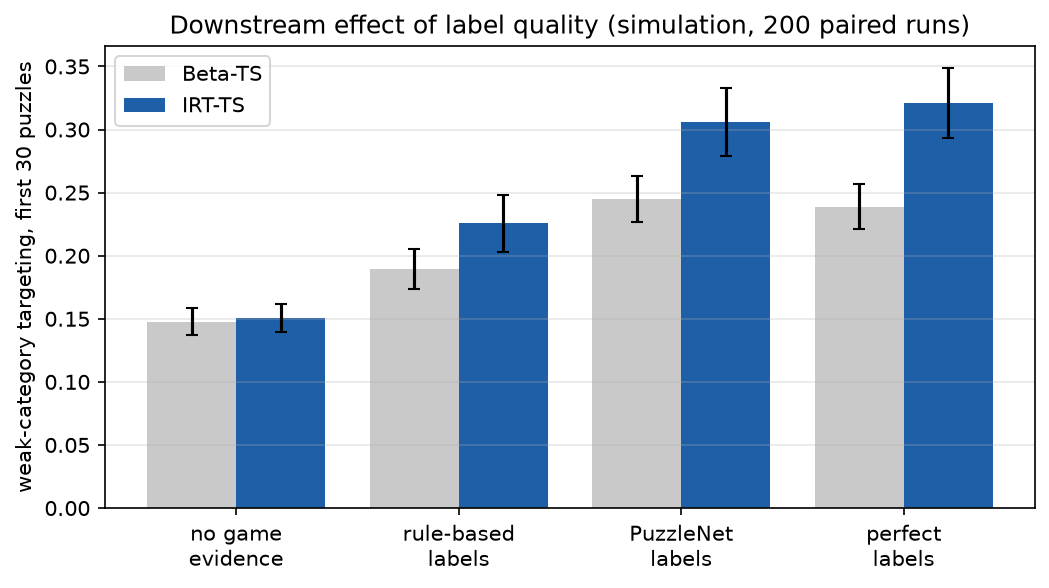
\includegraphics[width=0.8\linewidth]{figures/nn_label_simulation.png}
\caption{Downstream effect of label quality on early weak-category targeting (200 paired runs). PuzzleNet's labels are not statistically distinguishable from perfect ones.}\label{fig:nn-labelsim}
\end{figure}

\paragraph{Real players: the labels change, the diagnosis does not.} The 300-player cohort was
relabelled. Every one of the 40{,}067 critical positions was re-analysed with Stockfish at the
analyzer's own settings, and the resulting engine lines were labelled twice, once by each labeller, so
that the two versions of the cohort differ only in the labeller. Re-running the rule-based tagger on
the fresh engine lines reproduces its stored label 94.1\% of the time, which says the pipeline is
stable; the two labellers, however, agree with each other on only 37\% of real game positions. They
disagree about what players face:

\begin{table}[H]
\centering
\small
\caption{What the two labellers say the 40{,}067 critical positions of 300 real players
are.}\label{tab:nn-cohort-share}
\begin{tabularx}{\linewidth}{Xcc}
\toprule
\textbf{Category} & \textbf{Rule-based} & \textbf{PuzzleNet} \\
\midrule
Quiet Move        & 35\% & 12\% \\
General (no motif) & 11\% & 32\% \\
Endgame           & $<$1\% & 14\% \\
Fork              & 12\% & 5\% \\
Hanging Piece     & 9\% & 9\% \\
\bottomrule
\end{tabularx}
\end{table}

Given that the two labellers score $\kappa = 0.78$ and $0.49$ against an independent reference on
engine lines, the network's picture is the more credible: most critical positions in real games carry
no nameable motif, and a large share are endgame technique, while the rule-based tagger was calling a
third of everything a quiet move. That matters beyond this experiment, because the population category
norms shipped in the application (Section~\ref{sec:player-model}) were fitted on the rule-based
labels.

What does \emph{not} change is the conclusion of Section~\ref{sec:cohort-results}. With PuzzleNet
labels, split-half reliability of a player's per-category hit rates stays at zero (mean $|r| = 0.09$
across the categories with enough support, against $0.15$ before; the noise-corrected between-player
standard deviation is 0.0 under both labellings), and the ranking of the weakness models is unchanged.

\begin{finding}[Label noise was not the reason weaknesses looked like noise]
Tripling macro recall and nearly doubling $\kappa$ leaves per-category reliability at zero. The
earlier negative result therefore survives its most obvious challenge: it is not an artefact of a
crude labeller. From about 40 games, a player's per-category hit rates carry no stable
person-specific signal, whoever does the labelling, so personal weakness has to be learned online from
puzzle attempts rather than read off past games.
\end{finding}

\paragraph{Real logs: the difficulty estimate does not transfer to mined puzzles.} The third test is
the prequential replay of the application's own 123 attempts. Replacing the miner's formula with
PuzzleNet's difficulty makes the calibration \emph{worse}: log loss rises from 0.599 to 0.754.

The reason is visible in the numbers. For the 44 mined puzzles in the logs, PuzzleNet predicts a
difficulty 493 rating points higher on average than the formula (1611 against 1118), yet players solve
86.7\% of mined puzzles, against 80.0\% of Lichess pool puzzles. A mined puzzle is a position from the
player's \emph{own} game, which they have already seen at the board; it is easier for its owner than
its content suggests, and no model trained on Lichess ratings can know that. The formula's low ratings
were arbitrary, but they happened to sit closer to the truth for this population.

\begin{honest}[Honest status: the difficulty head is not used to serve mined puzzles]
The application records PuzzleNet's difficulty and uncertainty on every mined puzzle, but serves the
formula's rating unless \code{MINED\_RATING=puzzlenet} is set. Fitting the offset that would correct
the transfer needs data: a single scalar fitted on these 123 attempts runs to the edge of its range
(1181 points), which is fitting the 84.6\% base rate rather than the difficulty. The honest position
is that the difficulty head is well calibrated where it was validated --- Lichess puzzles, where its
intervals cover what they claim --- and unvalidated where the system would use it. The uncertainty it
reports is used: it is what a mined puzzle carries into the Bayesian update once the offset is known.
\end{honest}


\begin{figure}[H]
\centering
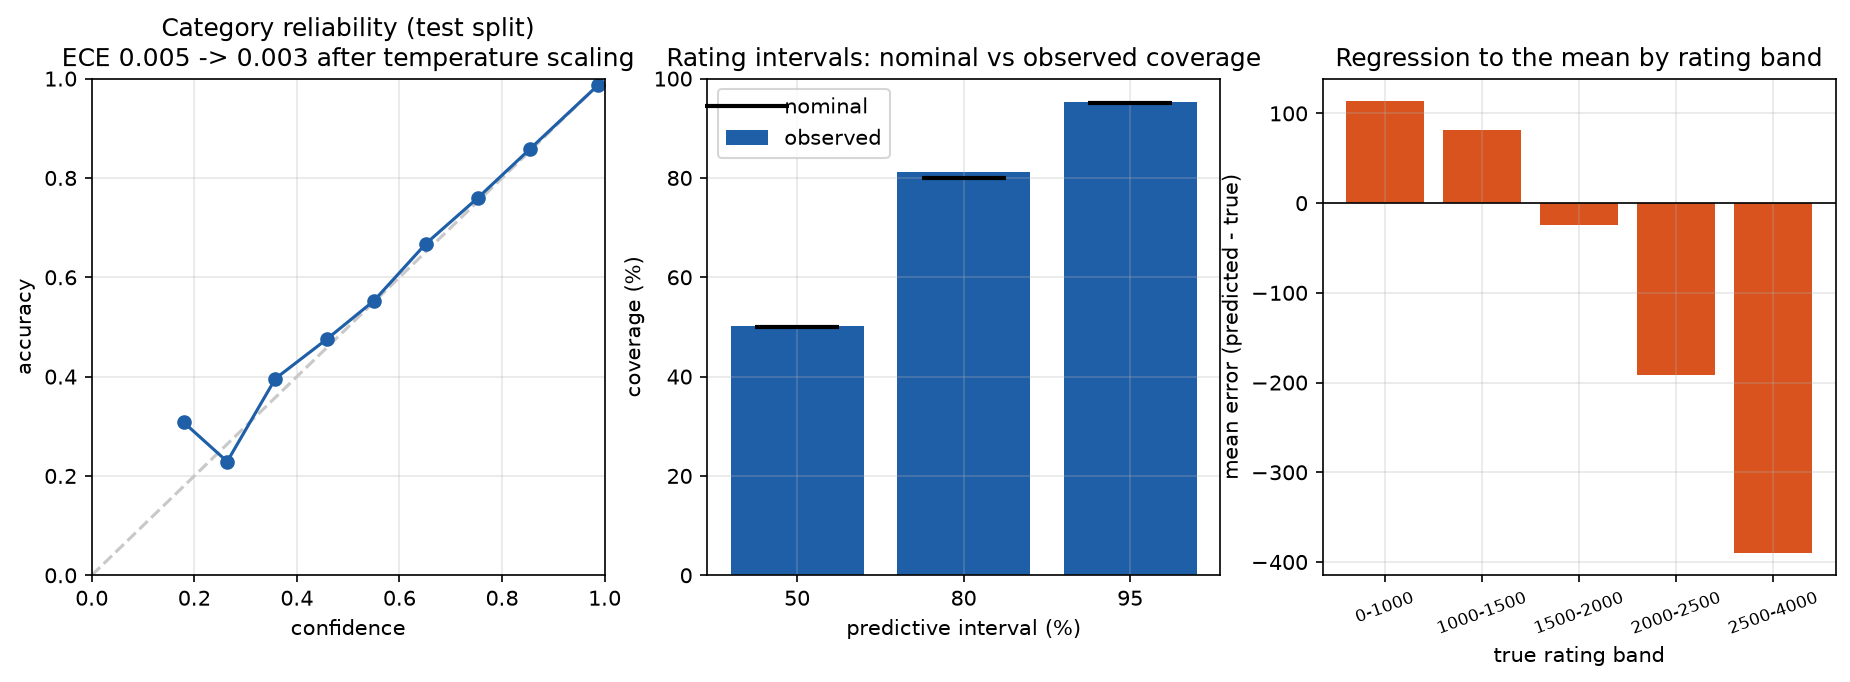
\includegraphics[width=\linewidth]{figures/nn_calibration.png}
\caption{Calibration on the test split. Left: category confidence against accuracy. Middle: how often the predicted difficulty intervals contain the Lichess rating, against what they claim. Right: the regression to the mean that a squared-error fit produces at the extremes.}\label{fig:nn-calibration}
\end{figure}


\subsection{Labelling engine lines, which is what the application actually does}\label{sec:nn-deployment}

Every number so far comes from puzzle solution lines. In the application the labeller sees something
else: Stockfish's principal variation from a critical position in a real game, cut to a fixed number
of plies. A puzzle solution stops when the tactic is complete; an engine line runs on into the won
position that follows. To measure that shift, 2{,}000 held-out harness puzzles were re-analysed with
the analyzer's own settings, and both labellers were scored on the engine line and on the solution
line of the same puzzles.

\begin{table}[H]
\centering
\small
\caption{Agreement with the Lichess category on 2{,}000 held-out puzzles, by the line the labeller is
shown. The engine's first move is the puzzle's first solution move in 99.3\% of these positions, so
the difference is about the line, not about the engine finding something else.}\label{tab:nn-engine}
\begin{tabularx}{\linewidth}{Xcc}
\toprule
\textbf{Line shown to the labeller} & \textbf{Strict agreement} & \textbf{$\kappa$} \\
\midrule
Rule-based tagger, puzzle solution        & 56.9\% & 0.504 \\
Rule-based tagger, engine line (7 plies)  & 55.5\% & 0.489 \\
\midrule
PuzzleNet, puzzle solution                & 91.9\% & 0.905 \\
PuzzleNet, engine line (1 ply)            & 66.4\% & 0.602 \\
PuzzleNet, engine line (3 plies)          & 80.3\% & 0.769 \\
\textbf{PuzzleNet, engine line (5 plies)} & \textbf{80.9\%} & \textbf{0.777} \\
PuzzleNet, engine line (7 plies)          & 76.5\% & 0.726 \\
\bottomrule
\end{tabularx}
\end{table}

\begin{honest}[Honest status: the network loses a third of its advantage in deployment]
PuzzleNet was trained on solution lines, so the engine line costs it a great deal: $\kappa$ falls from
0.91 to 0.78. The rule-based tagger barely moves (0.50 to 0.49), because it restricts which motifs may
be claimed at which depth and so ignores most of the continuation anyway. The deployed advantage is
therefore $\kappa = 0.78$ against $0.49$, not $0.91$ against $0.52$. It is still a large advantage,
and it is the honest one to quote for game analysis.
\end{honest}

The table also fixes a parameter. Agreement peaks when the network is shown five plies, and drops by
0.05 of $\kappa$ at seven, which is what the analyzer previously passed to the tagger. The deployed
system now gives the network the first five plies (\code{labeller.NEURAL\_PV\_PLIES}) and the
rule-based tagger the full line it was validated on. That is a measured choice, not a guess.

\subsection{What the network is actually learning: ablations}\label{sec:nn-ablations}

Every ablation trains on the same one-million-puzzle subset with the same schedule and is scored on
the same test split, so the rows differ only in what is named. The table is generated from
\code{eval/neural/puzzlenet\_evaluation.json} by \code{dissertation/build\_ablation\_table.py}, so it
cannot drift from the experiments.

\begin{table}[H]
\centering
\small
\caption{Ablations (1M training puzzles each) and the data-scaling sweep, all on the same test
split. $\kappa$ and macro-$F_1$ are the category head; RMSE is the difficulty head in rating points; a
dash means the model has no such head. Training times are not comparable across rows: the runs
shared a loaded laptop.}\label{tab:nn-ablations}
\begin{tabularx}{\linewidth}{Xcccc}
\toprule
\textbf{Variant} & \textbf{$\kappa$} & \textbf{Macro-$F_1$} & \textbf{RMSE} & \textbf{Train (s)} \\
\midrule
Reference: 512--256 trunk, all features, all heads & 0.867 & 0.774 & 285 & 516 \\
\midrule
No hidden layers (logistic / linear regression) & 0.743 & 0.610 & 326 & 294 \\
Raw boards and moves only & 0.741 & 0.645 & 313 & 505 \\
Hand-built relations only (no boards, no moves) & 0.830 & 0.708 & 305 & 74 \\
Wider trunk: 1024--512 & 0.878 & 0.797 & 280 & 4907 \\
\midrule
Category head alone (no multi-task) & 0.870 & 0.782 & --- & 486 \\
Difficulty head alone (no multi-task) & --- & --- & 280 & 468 \\
$\beta = 0$ (plain noise-aware likelihood) & 0.860 & 0.763 & 283 & 562 \\
$\beta = 1$ (squared-error gradient for the mean) & 0.868 & 0.777 & 289 & 250 \\
\midrule
30{,}000 training puzzles & 0.722 & 0.570 & 351 & 95 \\
100{,}000 & 0.780 & 0.654 & 333 & 127 \\
300{,}000 & 0.823 & 0.708 & 297 & 122 \\
1{,}000{,}000 & 0.867 & 0.774 & 285 & 516 \\
\textbf{5{,}526{,}626 (the production model)} & \textbf{0.914} & \textbf{0.861} & \textbf{268} & \textbf{2478} \\
\bottomrule
\end{tabularx}
\end{table}

\begin{finding}[Representation and data, not capacity]
The hand-built tactical relations carry most of the signal: on their own, with no boards and no move
blocks at all, they reach $\kappa = 0.830$ against $0.867$ for the full input. The raw boards and
moves on their own reach $0.741$. Each still adds something the other lacks --- the relations add
$0.126$ to the raw input, the raw input adds $0.037$ to the relations --- but a reader should not
conclude that the network has learned chess from squares. Depth matters about as much as the
relations: with no hidden layers, on the same features, $\kappa$ falls to $0.743$. Capacity is the
cheapest thing to buy and the least useful: four times the trunk buys $0.011$, while 5.5 times the
data buys $0.047$ and the curve has not flattened.
\end{finding}

\begin{figure}[H]
\centering
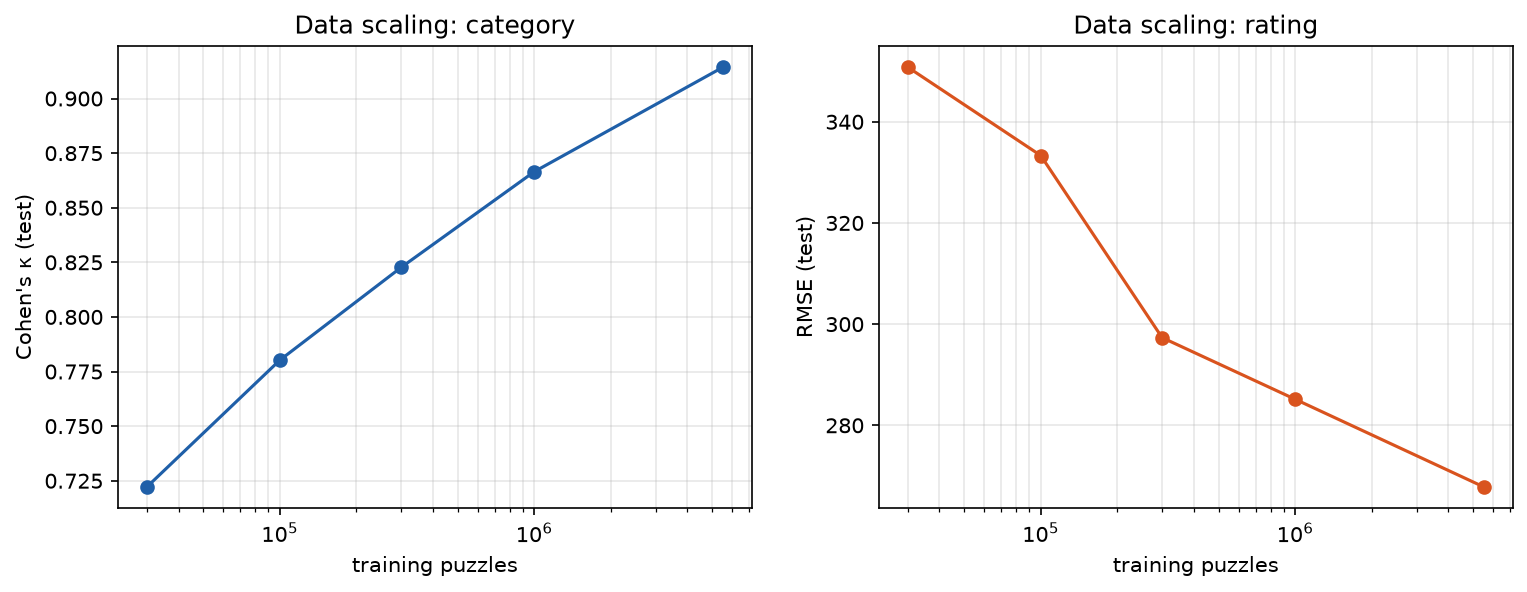
\includegraphics[width=\linewidth]{figures/nn_data_scaling.png}
\caption{Data scaling. Both heads keep improving to the full 5.5M puzzles; the curve has not flattened, so the model is limited by data rather than by capacity.}\label{fig:nn-scaling}
\end{figure}

Two results are negative and worth stating plainly. First, \textbf{multi-task learning does not help
either task here}: the category head alone reaches $\kappa = 0.870$ against $0.867$ when it shares a
trunk with themes and difficulty, and the difficulty head alone reaches RMSE 280 against 285. The
shared trunk costs a little on each task; what it buys is one model, one encoding pass and one file
instead of two, which is why the deployed model keeps it. Second, \textbf{the $\beta$-NLL correction
is not doing much work}. Plain noise-aware likelihood ($\beta = 0$) gives the best RMSE of the three
(283 against 285 at $\beta = 0.5$ and 289 at $\beta = 1$), and the differences are small either
way. The pathology that motivates
$\beta$-NLL~\cite{seitzer2022pitfalls} is that a learned variance can silence hard examples; here the
dominant part of the variance is the puzzle's \emph{known} rating deviation, and down-weighting a
noisily labelled puzzle is exactly the right thing to do, so the correction has little left to fix. On
another dataset without known label noise the argument for it would be stronger.


\subsection{Downstream: does better labelling help the recommender?}\label{sec:nn-downstream}

A labeller is only worth what it changes. Three downstream tests follow, one simulated and two on real
data, and they do not all point the same way.

\paragraph{Simulation: the label-quality bottleneck closes.} Experiment E3
(Section~\ref{sec:ablations}) measured how much early weak-category targeting depends on label
quality, by drawing each observed label from the labeller's measured $P(\text{predicted} \mid
\text{true})$. Rerunning it with PuzzleNet's confusion matrix, on the same 200 seeds so that every
comparison is paired:

\begin{table}[H]
\centering
\small
\caption{Weak-category targeting over the first 30 puzzles, by the source of the game evidence
(200 paired runs, $T = 60$).}\label{tab:nn-labelsim}
\begin{tabularx}{\linewidth}{Xcc}
\toprule
\textbf{Label source} & \textbf{Beta-TS} & \textbf{IRT-TS} \\
\midrule
No game evidence              & 0.148 & 0.151 \\
Rule-based tagger             & 0.189 & 0.226 \\
\textbf{PuzzleNet}            & \textbf{0.245} & \textbf{0.306} \\
Perfect labels                & 0.239 & 0.321 \\
\bottomrule
\end{tabularx}
\end{table}

\begin{finding}[PuzzleNet labels are statistically indistinguishable from perfect ones]
For the IRT policy, PuzzleNet beats the rule-based tagger by $+0.080$ targeting
(95\% CI $+0.055$ to $+0.105$, $p = 7 \times 10^{-10}$, $d_z = 0.46$), and the remaining gap to
\emph{perfect} labels is $+0.015$ and not significant ($p = 0.31$). It closes 84\% of the
rules-to-perfect gap for IRT-TS and all of it for Beta-TS. Cumulative regret falls from 62.6 to 55.3,
against 53.2 with perfect labels. The bottleneck identified in E3 is, in simulation, gone.
\end{finding}

\begin{figure}[H]
\centering
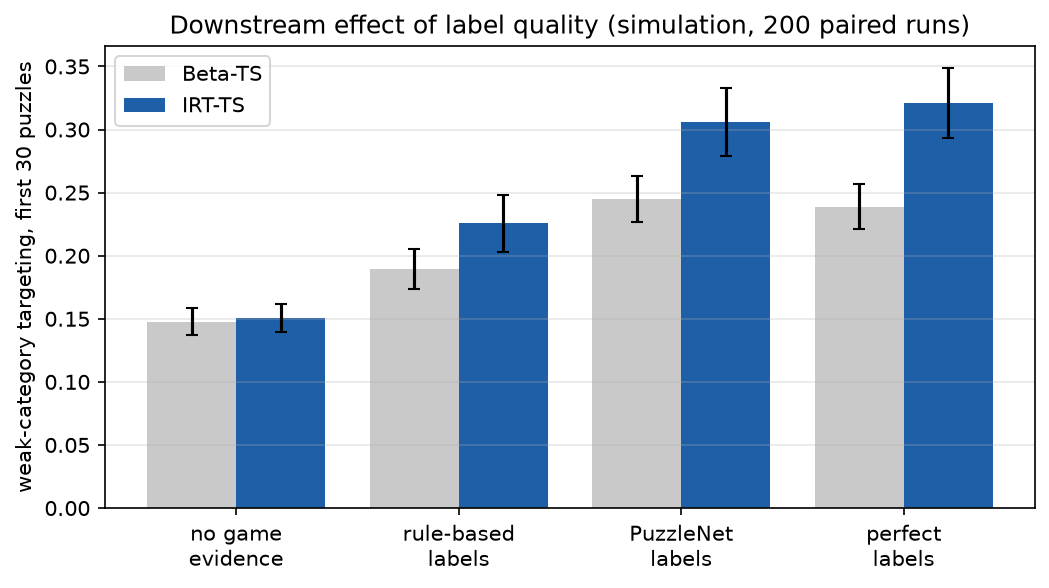
\includegraphics[width=0.8\linewidth]{figures/nn_label_simulation.png}
\caption{Downstream effect of label quality on early weak-category targeting (200 paired runs). PuzzleNet's labels are not statistically distinguishable from perfect ones.}\label{fig:nn-labelsim}
\end{figure}

\paragraph{Real players: the labels change, the diagnosis does not.} The 300-player cohort was
relabelled. Every one of the 40{,}067 critical positions was re-analysed with Stockfish at the
analyzer's own settings, and the resulting engine lines were labelled twice, once by each labeller, so
that the two versions of the cohort differ only in the labeller. Re-running the rule-based tagger on
the fresh engine lines reproduces its stored label 94.1\% of the time, which says the pipeline is
stable; the two labellers, however, agree with each other on only 37\% of real game positions. They
disagree about what players face:

\begin{table}[H]
\centering
\small
\caption{What the two labellers say the 40{,}067 critical positions of 300 real players
are.}\label{tab:nn-cohort-share}
\begin{tabularx}{\linewidth}{Xcc}
\toprule
\textbf{Category} & \textbf{Rule-based} & \textbf{PuzzleNet} \\
\midrule
Quiet Move        & 35\% & 12\% \\
General (no motif) & 11\% & 32\% \\
Endgame           & $<$1\% & 14\% \\
Fork              & 12\% & 5\% \\
Hanging Piece     & 9\% & 9\% \\
\bottomrule
\end{tabularx}
\end{table}

Given that the two labellers score $\kappa = 0.78$ and $0.49$ against an independent reference on
engine lines, the network's picture is the more credible: most critical positions in real games carry
no nameable motif, and a large share are endgame technique, while the rule-based tagger was calling a
third of everything a quiet move. That matters beyond this experiment, because the population category
norms shipped in the application (Section~\ref{sec:player-model}) were fitted on the rule-based
labels.

What does \emph{not} change is the conclusion of Section~\ref{sec:cohort-results}. With PuzzleNet
labels, split-half reliability of a player's per-category hit rates stays at zero (mean $|r| = 0.09$
across the categories with enough support, against $0.15$ before; the noise-corrected between-player
standard deviation is 0.0 under both labellings), and the ranking of the weakness models is unchanged.

\begin{finding}[Label noise was not the reason weaknesses looked like noise]
Tripling macro recall and nearly doubling $\kappa$ leaves per-category reliability at zero. The
earlier negative result therefore survives its most obvious challenge: it is not an artefact of a
crude labeller. From about 40 games, a player's per-category hit rates carry no stable
person-specific signal, whoever does the labelling, so personal weakness has to be learned online from
puzzle attempts rather than read off past games.
\end{finding}

\paragraph{Real logs: the difficulty estimate does not transfer to mined puzzles.} The third test is
the prequential replay of the application's own 123 attempts. Replacing the miner's formula with
PuzzleNet's difficulty makes the calibration \emph{worse}: log loss rises from 0.599 to 0.754.

The reason is visible in the numbers. For the 44 mined puzzles in the logs, PuzzleNet predicts a
difficulty 493 rating points higher on average than the formula (1611 against 1118), yet players solve
86.7\% of mined puzzles, against 80.0\% of Lichess pool puzzles. A mined puzzle is a position from the
player's \emph{own} game, which they have already seen at the board; it is easier for its owner than
its content suggests, and no model trained on Lichess ratings can know that. The formula's low ratings
were arbitrary, but they happened to sit closer to the truth for this population.

\begin{honest}[Honest status: the difficulty head is not used to serve mined puzzles]
The application records PuzzleNet's difficulty and uncertainty on every mined puzzle, but serves the
formula's rating unless \code{MINED\_RATING=puzzlenet} is set. Fitting the offset that would correct
the transfer needs data: a single scalar fitted on these 123 attempts runs to the edge of its range
(1181 points), which is fitting the 84.6\% base rate rather than the difficulty. The honest position
is that the difficulty head is well calibrated where it was validated --- Lichess puzzles, where its
intervals cover what they claim --- and unvalidated where the system would use it. The uncertainty it
reports is used: it is what a mined puzzle carries into the Bayesian update once the offset is known.
\end{honest}



\section{Evaluation of Style-Conditional Generation}\label{sec:rating-classifier}

\begin{honest}[Honest status]
Style-conditional puzzle generation could not be evaluated, because no generative model was built
(Section~\ref{sec:generation}). This section instead evaluates the two player-modelling claims the
system relies on, on real players: that a player's level can be read from how they play (RQ1), and
that their tactical weaknesses can be diagnosed from their games (RQ2).
\end{honest}

\subsection{Rating-group classification (Objective O1)}

\begin{table}[H]
\centering
\small
\caption{Rating-band classification, 300 players, 5 bands, chance 20\%.}\label{tab:rating}
\begin{tabular}{lrrrr}
\toprule
\textbf{Model} & \textbf{Accuracy} & \textbf{Macro-F1} & \textbf{Within one band} & \textbf{Permutation $p$} \\
\midrule
Logistic regression & $59.1\% \pm 1.8$ & 0.588 & 93.1\% & 0.002 \\
Random forest & $57.4\% \pm 1.9$ & 0.570 & 93.8\% & 0.002 \\
\bottomrule
\end{tabular}
\end{table}

A player's rating band is predicted from how they play at almost three times chance. The prediction
is within one band 93\% of the time, and no information about ratings is used. The permutation $p$ of
0.002 is the smallest attainable with 500 shuffles: no shuffled labelling reached the observed
accuracy. Viewed as regression, the rating itself is predicted with a mean absolute error of 206
rating points, against 490 for predicting the mean ($r = 0.895$). The most important features are mean
win-probability loss, mean centipawn loss, median win-probability loss, the critical-position hit rate
and blunders per game.

\begin{figure}[H]
\centering
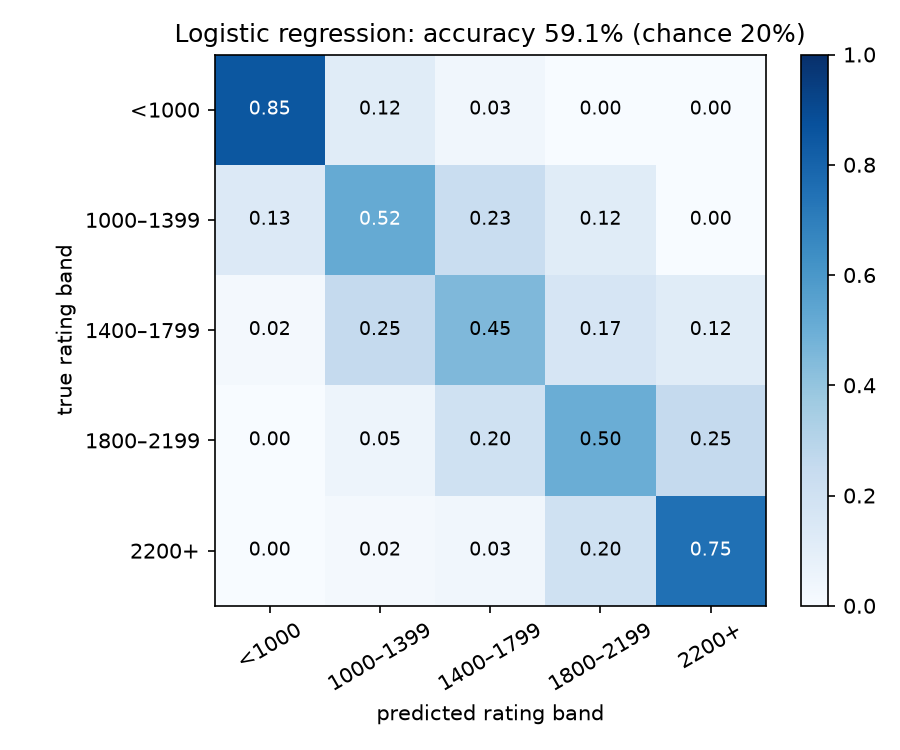
\includegraphics[width=0.58\linewidth]{figures/rating_band_confusion.png}
\caption{Row-normalised confusion matrix of the logistic-regression classifier. Errors fall almost
entirely in adjacent bands.}\label{fig:rating}
\end{figure}

\subsection{Diagnosing tactical weaknesses on real players}\label{sec:cohort-results}

Each player's oldest two-thirds of games are used to predict the critical positions they miss in their
newest third: 11,973 held-out opportunities in total. Population parameters are always fitted on other
players (5-fold, grouped by player).

\begin{table}[H]
\centering
\small
\caption{Predicting future misses (300 players). $\Delta$LL is relative to the category base rate;
negative is better.}\label{tab:cohort}
\begin{tabular}{lrrrr}
\toprule
\textbf{Model} & \textbf{Log loss} & \textbf{AUC} & $\boldsymbol{\Delta}$\textbf{LL [95\% CI]} & \textbf{Top-3 recall} \\
\midrule
Global base rate & 0.6545 & 0.494 & $+0.0145$ [$+0.011$, $+0.018$] & 0.60 \\
Category base rate & 0.6401 & 0.582 & reference & 0.71 \\
Player base rate & 0.6491 & 0.568 & $+0.0091$ [$+0.004$, $+0.015$] & 0.60 \\
Rule-based scorer (original) & 0.6547 & 0.474 & $+0.0147$ [$+0.011$, $+0.018$] & 0.59 \\
RF trained on simulated players & 0.6529 & 0.505 & $+0.0128$ [$+0.009$, $+0.016$] & 0.62 \\
EB, shrink to player rate & 0.6506 & 0.582 & $+0.0105$ [$+0.005$, $+0.016$] & 0.66 \\
\textbf{EB, shrink to population norms} & \textbf{0.6326} & \textbf{0.620} & $\mathbf{-0.0074}$ [$-0.012$, $-0.003$] & 0.70 \\
RF trained on real players & 0.6321 & 0.618 & $-0.0080$ [$-0.012$, $-0.005$] & 0.71 \\
\bottomrule
\end{tabular}
\end{table}

Three results stand out:
\begin{enumerate}
  \item \textbf{The original rule-based scorer and the random forest trained on simulated players carry
        no usable information} about a real player's future misses (AUC 0.47 and 0.51). This is the
        circularity risk from training on synthetic data, made concrete.
  \item \textbf{Only two models beat population base rates}, and they are statistically tied:
        shrinkage towards population norms (used in production, because it needs no training and is
        interpretable) and a random forest trained on real players. The margins are small.
  \item \textbf{Per-category weakness barely replicates within a player.} Cross-validation chose a
        shrinkage strength of 128--256 pseudo-opportunities. Split-half reliability is near zero for
        most categories: Fork $r=0.08$ ($n=227$ players), Quiet Move $0.03$ ($n=299$), Hanging Piece
        $-0.06$ ($n=148$). The noise-corrected spread of personal category deviations is estimated at
        zero. There is also no family structure: within-family correlation is $-0.08$, against $-0.12$
        across families.
\end{enumerate}

\begin{finding}[Key finding: weakness diagnosis]
With about 40 games of history (roughly 80 critical positions spread over 15 or more categories), a
player's category-specific weaknesses cannot be separated from sampling noise. The reliable signals are
the player's overall level and how hard each motif is for everyone. This directly challenges the
premise of every ``mistakes from your games'' trainer. It also shows why the system must learn personal
weaknesses \emph{online}, from targeted puzzle attempts.
\end{finding}

\section{Adaptive vs Non-Adaptive Training Comparison}

\subsection{E1: pre-registered replication}

The protocol was fixed before any results existed: three categories solved 30\% of the time, twenty at
80\%, 200 runs of 150 attempts, uniform priors, and the original Beta-TS.

\begin{table}[H]
\centering
\small
\caption{Pre-registered criteria for the original Beta-TS bandit.}\label{tab:e1}
\begin{tabular}{llll}
\toprule
\textbf{Criterion} & \textbf{Threshold} & \textbf{Result [95\% CI]} & \\
\midrule
C1 targeting, trials 131--150 & $\geq 80\%$ & 71.4\% [69.5, 73.2] & \textbf{fail} \\
C2 posterior MAE at trial 100 & $\leq 0.10$ & 0.111 [0.108, 0.114] & \textbf{fail} \\
C3 vs random (Welch's $t$) & $p<0.01$, $d>0.8$ & $p<10^{-100}$, $d=5.4$ & pass \\
\bottomrule
\end{tabular}
\end{table}

The bandit is far better than random, but misses two thresholds that were set without accounting for
the cost of exploration. Thompson Sampling keeps sampling the 20 strong arms, which lowers targeting
and leaves their estimates noisy (Figure~\ref{fig:e1}). The greedy policy reaches 100\% targeting here,
but only because the weak arms are unambiguous; it collapses once the player learns (E2).

\begin{figure}[H]
\centering
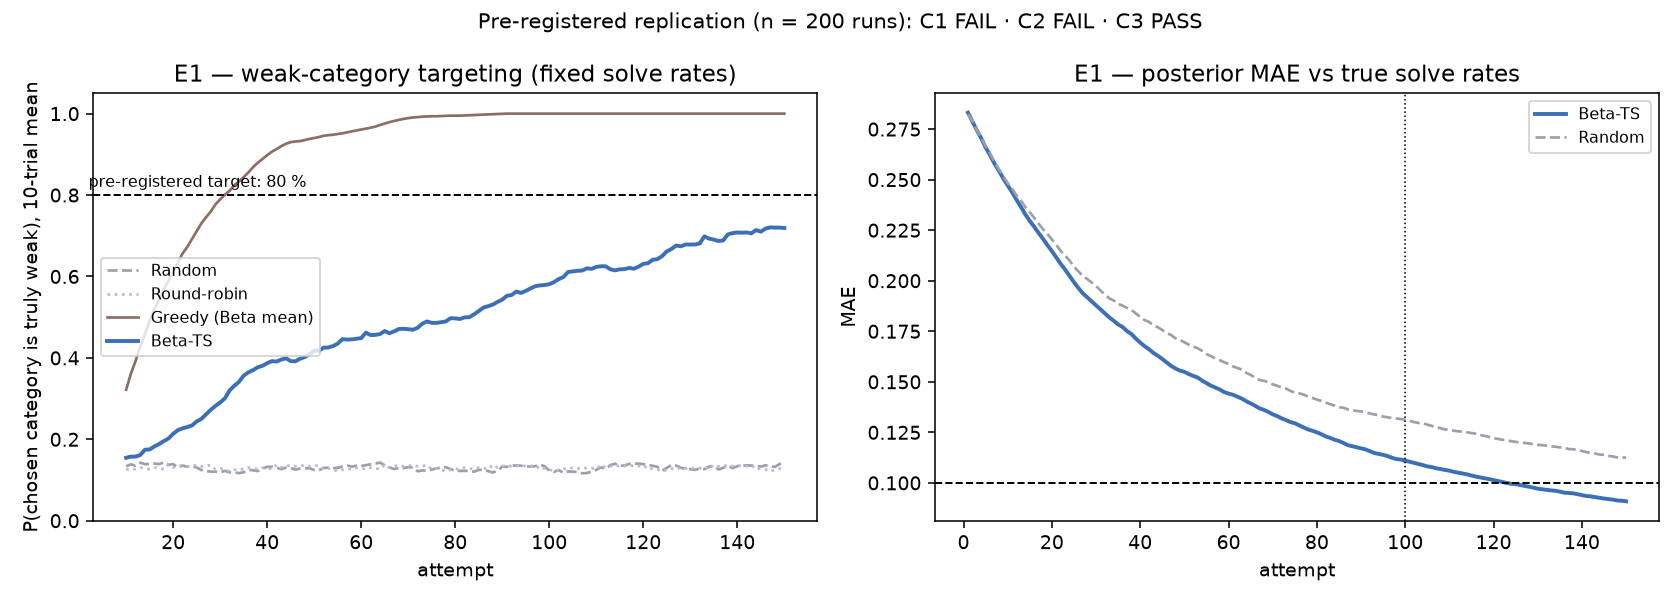
\includegraphics[width=\linewidth]{figures/e1_preregistered.png}
\caption{E1: targeting (left) and posterior MAE (right) over 150 attempts.}\label{fig:e1}
\end{figure}

\subsection{E2: semi-synthetic comparison}

Synthetic players have a known $\theta$ and $\delta$. Three categories are weak by about 210 rating
points. Puzzle difficulties are drawn from the real Lichess distribution for each category. The
player's Elo is only a noisy guide to puzzle ability, and the evidence from games is mislabelled
according to the measured confusion matrix of the new tagger.

\begin{table}[H]
\centering
\small
\caption{E2, no learning, 200 paired runs.}\label{tab:e2}
\begin{tabular}{lrrrrr}
\toprule
\textbf{Policy} & \textbf{Targeting (last 50)} & \textbf{Regret} & \textbf{Frustrating} & \textbf{Productive} & \textbf{Top-3} \\
\midrule
Random & 0.130 & 189.2 & 33.8\% & 37\% & 0.40 \\
Round-robin & 0.132 & 189.1 & 33.6\% & 37\% & 0.41 \\
Static profile & 0.206 & 166.6 & 35.8\% & 36\% & 0.26 \\
Greedy & 0.520 & 103.5 & 49.3\% & 25\% & 0.26 \\
Beta-TS (original) & 0.404 & 145.9 & 44.1\% & 29\% & 0.45 \\
Beta-TS, $\gamma=0.97$ & 0.244 & 164.9 & 39.8\% & 32\% & 0.35 \\
IRT-TS, Elo band & 0.409 & 142.3 & 42.5\% & 31\% & 0.49 \\
\textbf{IRT-TS (new)} & \textbf{0.445} & \textbf{135.9} & \textbf{3.2\%} & \textbf{72\%} & \textbf{0.49} \\
Oracle & 1.000 & 0.0 & 0.0\% & 82\% & 1.00 \\
\bottomrule
\end{tabular}
\end{table}

Paired against Beta-TS, IRT-TS reduces regret by 10.0 (95\% CI [$-15.3$, $-4.8$], $p_\text{Holm} <
0.001$). It cuts the share of frustrating puzzles by 41 points ($d_z = -2.52$). Its targeting gain of
$+0.041$ ([0.002, 0.081]) is \emph{not} significant after Holm correction ($p_\text{Holm}=0.089$). All
adaptive policies beat random decisively (Beta-TS against random: $d_z = 1.19$ on targeting).

\begin{figure}[H]
\centering
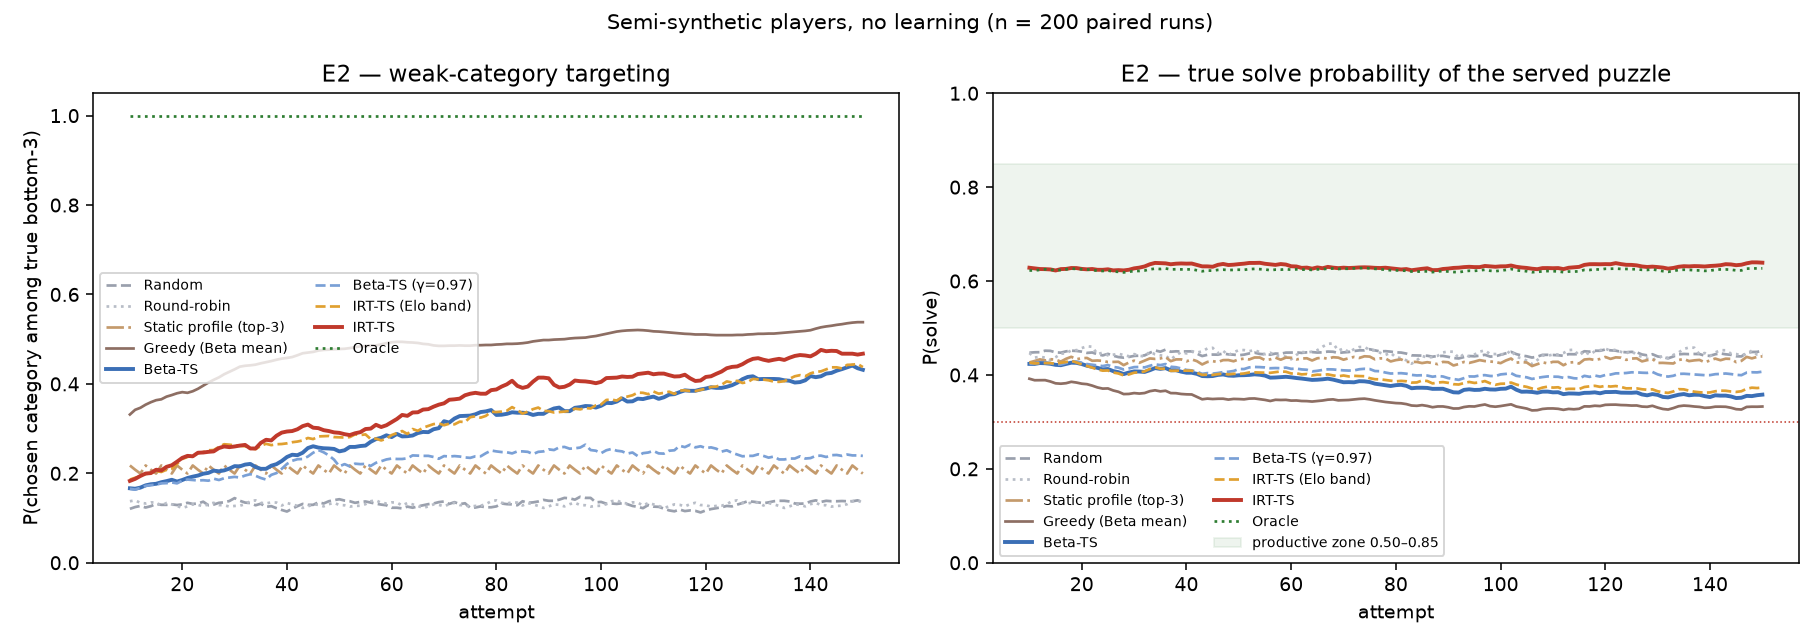
\includegraphics[width=\linewidth]{figures/e2_targeting_and_difficulty.png}
\caption{E2: targeting over time (left) and the true solve probability of each served puzzle (right).
IRT-TS matches the Oracle's difficulty inside the productive zone.}\label{fig:e2}
\end{figure}

\paragraph{Learning gain depends on the assumed learning mechanism.} A simulated learning gain follows
from an \emph{assumed} learning model, so two are reported. Under ``zpd'', learning is greatest on
puzzles near the edge of ability. Under ``error'', players learn from seeing the solution after a miss.

\begin{table}[H]
\centering
\small
\caption{Gain in the initially weak categories (logits), with the paired difference against Beta-TS.}\label{tab:gain}
\begin{tabular}{lrrrl}
\toprule
\textbf{Learning model} & \textbf{Random} & \textbf{Beta-TS} & \textbf{IRT-TS} & \textbf{IRT $-$ Beta [95\% CI]} \\
\midrule
zpd & 0.256 & 0.543 & 0.675 & $+0.133$ [0.092, 0.174], $d_z = 0.45$ \\
error & 0.284 & 0.516 & 0.386 & $-0.130$ [$-0.163$, $-0.098$], $d_z = -0.53$ \\
\bottomrule
\end{tabular}
\end{table}

\begin{figure}[H]
\centering
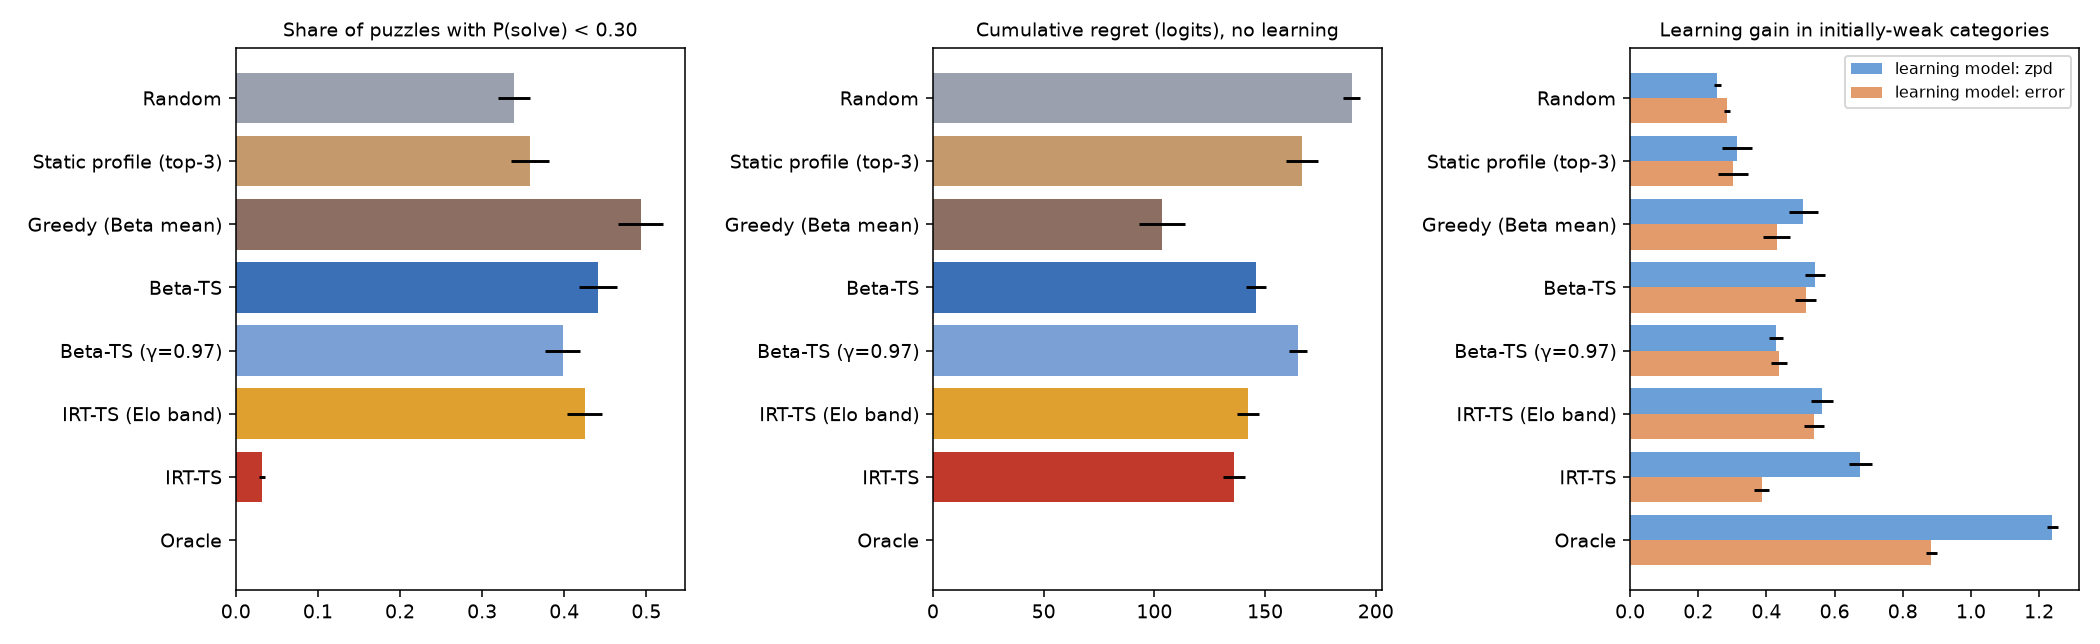
\includegraphics[width=\linewidth]{figures/e2_summary.png}
\caption{Frustration, regret and learning gain by policy, with 95\% confidence intervals.}\label{fig:e2summary}
\end{figure}

\section{Analysis of Results and Ablation Studies}\label{sec:ablations}

\paragraph{Where does the improvement come from?} The ablation \emph{IRT-TS, Elo band} uses the new
category selection with the old difficulty band. It performs like Beta-TS on every metric. The new
policy's benefit therefore comes almost entirely from \emph{difficulty targeting}, not from how it
chooses categories. This also explains the sign flip in Table~\ref{tab:gain}: easier, well-pitched
puzzles produce fewer failures, which helps under the zpd model and hurts under the error model.

\paragraph{E3: does label quality matter?} Early targeting (first 30 attempts) for IRT-TS rises from
0.151 with no game evidence, to 0.201 with the old labeller's errors, 0.226 with the new tagger's, and
0.321 with perfect labels. In paired comparisons, game evidence helps (new against none $+0.075$,
$p<10^{-9}$). Perfect labels would help much more (perfect against new $+0.095$, $p<10^{-9}$). The
improvement from old to new tagger is small and not significant ($+0.025$, $p=0.06$). Better labels are
necessary, but this tagger has not yet recovered most of the available gain.

\begin{figure}[H]
\centering
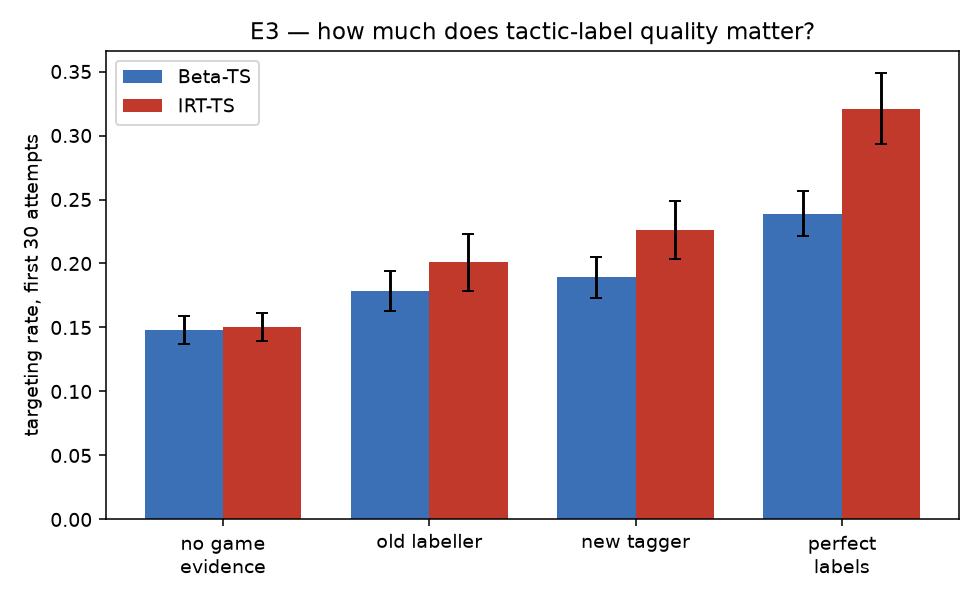
\includegraphics[width=0.7\linewidth]{figures/e3_label_quality.png}
\caption{E3: early targeting under four qualities of game evidence.}\label{fig:e3}
\end{figure}

\paragraph{E4: the player improves mid-session.} At attempt 75, the worst category improves by 1.5
logits. Discounted Thompson Sampling~\cite{raj2017taming} \emph{raises} regret after the change: by 19.2
at $\gamma=0.97$ ($d_z = 0.82$) and by 26.1 at $\gamma=0.93$ ($d_z = 1.01$). With 23 arms and few
attempts on each, forgetting every arm costs more than forgetting the one that changed. Discounting
therefore stays off. The IRT learner's random-walk drift is on a par with Beta-TS ($-1.4$, not
significant).

\begin{figure}[H]
\centering
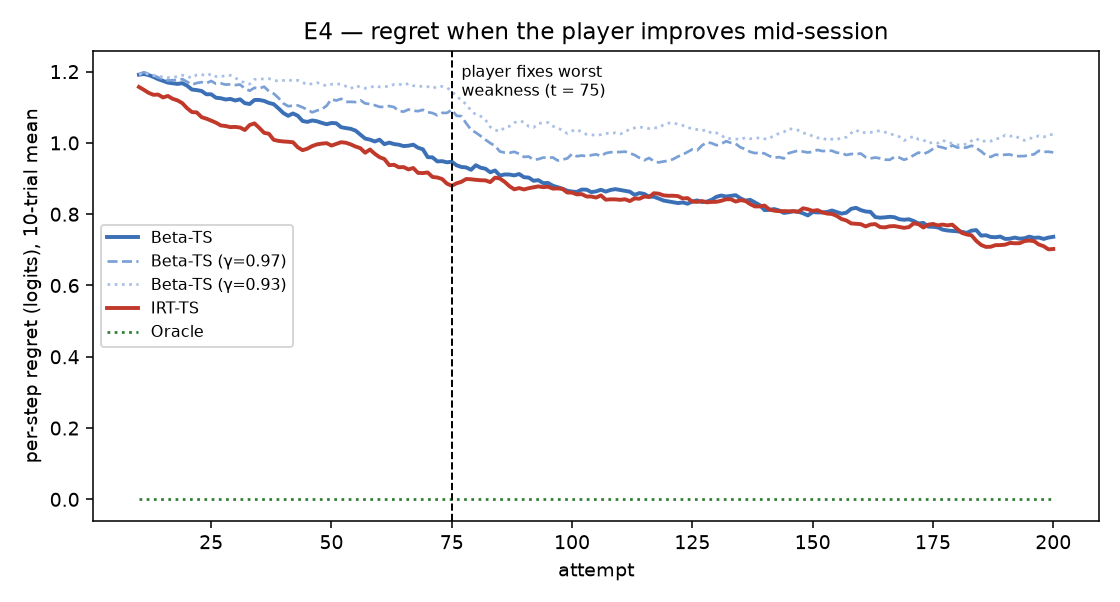
\includegraphics[width=0.75\linewidth]{figures/e4_changepoint.png}
\caption{E4: per-attempt regret around the change point.}\label{fig:e4}
\end{figure}

\paragraph{E5: sensitivity.} Beta-TS is insensitive to prior strength; targeting ranges from 0.361 to
0.406 across a tenfold range. For IRT-TS, targets of $p^\star=0.5$ and $0.65$ give the same targeting
(0.446 and 0.445), while $0.8$ is worse (0.409), because puzzles that are too easy carry little
information. Under the zpd model the gain is largest at $p^\star=0.5$. That is built into the
assumption, and $0.65$ is a compromise with frustration.

\paragraph{E6: family-structured prior.} A prior that correlates related motifs gives a small early
targeting gain ($+0.018$, $p=0.003$) and a small reduction in regret when weaknesses really do cluster
($-2.9$, $p=0.04$). The real cohort shows no clustering, so the option stays off.

\paragraph{E7: realistic effect sizes.} Calibrated on the cohort, with subtle weaknesses of $-0.5$
logits against a background of $0.15$, the advantage of Beta-TS over random shrinks from $+0.29$ to
$+0.10$ ($d_z = 0.55$), and IRT-TS's extra targeting edge over Beta-TS disappears ($+0.001$,
$p=0.95$). The reduction in frustrating puzzles holds in every world: from 35\% to 1.4\% with subtle
weaknesses, and from 28\% to 0.9\% with none at all ($d_z$ between $-1.7$ and $-2.6$). It is the most
robust result in the study.

\section{Threats to Validity}\label{sec:validity}

\paragraph{Internal validity.} No puzzle of the held-out harness entered PuzzleNet's training or its
model selection, and the rule-based numbers recomputed on that harness reproduce the published ones
exactly, which is evidence that both labellers were scored on identical data. Two gaps remain. The
network is trained on puzzle solution lines but deployed on engine lines, so its labelling accuracy in
the application is the engine-line figure of Section~\ref{sec:nn-deployment}, not the harness figure.
And its difficulty head is calibrated on Lichess puzzles, while it is used on puzzles mined from a
player's own games, for which no ground truth exists at all.

\paragraph{Internal validity of the simulations.} The simulated players use the same logistic model family as the IRT
learner, which favours it. The E2 ablation shows that the advantage comes from difficulty targeting,
which any correctly specified model would provide, but the favour remains. Learning gains depend
entirely on the assumed learning mechanism, which is why two are reported.

\paragraph{Construct validity.} Targeting a weak category is not the same as learning. Lichess themes
are an automatic reference, not ground truth, and this matters more now that a network is trained
\emph{to reproduce them}: PuzzleNet's $\kappa$ of \KAPPANN{} says it has learned Lichess's own tagger
almost exactly, not that either is right. Where the two taggers agree and both are wrong, nothing in
this evaluation can see it. A human-labelled sample would be needed to separate the two claims, and
none exists here. The opportunity definition (a gap of at least 10
win-percentage points, no recaptures) is a design choice, and other thresholds would change the
counts.

\paragraph{External validity.} The cohort is not a uniform random sample. Snowball and titled-player
sampling over-represent connected and titled players in the upper bands. Only rapid and blitz games
from Chess.com are used. The real puzzle logs come from five users, two of whom contribute most of the
attempts.

\paragraph{Statistical conclusion validity.} Many comparisons are made. Holm correction is applied
within each family of comparisons but not across experiments. The prequential analysis has only 123
events, so its confidence intervals are wide. The permutation $p$ of 0.002 is the floor of a
500-shuffle test, not an exact value.

\chapter{Discussion}\label{ch:discussion}

\section{Interpretation of Key Findings}

\paragraph{Adaptive difficulty is the robust result.} Across every simulated world, including one with
no category weaknesses at all, the difficulty-aware policy almost eliminates puzzles the player has
little chance of solving (from 28--45\% down to 1--3\%). It keeps most practice in the productive zone.
On the real logs, the assumption that difficulty could be pitched from the player's Chess.com rating
proved badly wrong (a predicted 45\% solve rate against 84.6\% observed). A model that learns the
player's puzzle ability online fixes this. These two facts support each other. Pitching difficulty
correctly is both the most reliable benefit and the one most directly checked against real data.

\paragraph{Weakness targeting is real, but small and fragile.} Adaptive category selection beats random
selection in every simulation. The advantage shrinks by about two-thirds when weaknesses are as subtle
as the real cohort suggests. The new policy's \emph{extra} targeting edge over the original bandit does
not survive realistic effect sizes. The pre-registered replication tells the same story: the original
bandit clearly beats random, but falls short of the targeting threshold it was held to.

\paragraph{Game histories reveal level, not weaknesses.} This is the most consequential finding. From
how a player plays, their rating band can be predicted at almost three times chance, and their rating
within about 200 points. Yet which tactical categories they will miss in future games is barely more
predictable than population base rates. Per-category reliability is near zero. Two explanations fit.
Either category-specific differences between players are genuinely small, compared with overall
strength and with how hard each motif is for everyone. Or the measurement is too noisy to reveal them:
about 80 critical positions per player, spread over many categories, labelled by a tagger with $\kappa
\approx 0.5$. Both lead to the same design conclusion. A player's games can supply only a weak prior on
\emph{which} motif to train. Personal weaknesses have to be learned online, from targeted puzzles, and
that is what the IRT learner does.

\paragraph{What the negative results mean for the original plan.} The portfolio's gap was puzzle
\emph{generation} conditioned on the learner's weaknesses. The cohort result bears directly on it. If
per-category weakness cannot be reliably measured from typical game histories, a generator conditioned
on a diagnosed weakness would largely be conditioned on noise. The change of direction towards
difficulty-aware selection, with weakness learned online, is therefore supported by evidence, and was
not only a response to limited compute.

\section{Relation to Prior Work}

The finding that level is detectable from play is consistent with behavioural stylometry, which
identifies individuals from their games~\cite{mcilroyyoung2021detecting}. It is also consistent with
Maia's finding that play varies systematically with rating~\cite{mcilroyyoung2020aligning}. Those
models use hundreds of games and deep sequence encoders; with only 18 hand-made features and 60 games
per player, level is still recoverable. By contrast, the weak per-category signal agrees with Hristova
et al.~\cite{hristova2014assessing}, who found that difficulty comes mainly from the depth of
calculation rather than recognising the motif. A taxonomy by motif may simply not be where players
differ most. The case for learning online rather than profiling up front matches the tutoring-bandit
literature~\cite{clement2015multi} and Elo-based adaptive systems~\cite{pelanek2016applications}, which
estimate learner and item parameters jointly from interactions. Nie et al.~\cite{nie2026discovering}
point the same way at a much larger scale: they learn puzzle value from 1.5 billion interactions, not
from game analysis. Feng et al.~\cite{feng2025generating} remain the reference for puzzle
\emph{creation}, which this work did not attempt.

\section{Limitations of the Current Approach}\label{sec:limitations}

\subsection{How sophisticated is the AI in this system? An honest assessment}

\begin{table}[H]
\centering
\small
\caption{The AI components, how they work, and how much they contribute.}\label{tab:ai-honest}
\begin{tabularx}{\linewidth}{p{0.24\linewidth}p{0.22\linewidth}p{0.1\linewidth}Y}
\toprule
\textbf{Component} & \textbf{Technique} & \textbf{Learned?} & \textbf{Honest assessment} \\
\midrule
IRT learner with Thompson Sampling & Online Bayesian logistic model, full-covariance Laplace update & Online, from every attempt & The most sophisticated component and the core contribution. Mathematically careful (reduces to Glicko; tested), but a known family of models (Elo, IRT, extended Kalman) applied to a new problem. \\
PuzzleNet & Multi-task neural network (3{,}329 features, 512--256 trunk, three heads), written and differentiated by hand in NumPy & Offline, from 5.5M Lichess puzzles & The only deep-learning component, and the largest single jump in measured quality: tactic labelling improves from $\kappa=0.52$ to \KAPPANN{} on the same held-out puzzles, and mined-puzzle difficulty acquires a calibrated estimate with an uncertainty attached. It is still a feed-forward network over an engineered representation, not a convolutional or attention model over raw boards, and its labels imitate another automatic tagger rather than human judgement. \\
Beta--Bernoulli bandit & Thompson Sampling & Online & Textbook; a few lines of code. \\
Rating-band classifier & Logistic regression, random forest & From 300 real players & Standard supervised learning. Solid result, simple models. \\
Weakness models & Empirical Bayes; random forest & From 300 real players & Classical statistics. Shows only a small advantage over base rates (Chapter~\ref{ch:results}). \\
Glicko-2 fitter & Bayesian rating system & From logs & A faithful re-implementation of a published algorithm. \\
Tactic tagger, miner gates & Hand-written rules over engine output & No & Symbolic AI. Measured and much improved, but engineered, not learned. \\
Stockfish & Alpha-beta search with an NNUE evaluator & Pre-trained (third party) & By far the strongest AI in the system, and not a contribution of this project. \\
Generative model / deep RL & --- & --- & \textbf{Still none.} No puzzle generator was trained and no policy was learned by reinforcement learning; the bandit and the IRT learner are Bayesian, not deep. \\
\bottomrule
\end{tabularx}
\end{table}

In summary, the AI here is \textbf{mostly classical and statistically principled, with one trained
neural component}. PuzzleNet is a genuine supervised deep-learning model: 1.86M parameters, a
hand-derived backward pass, a noise-aware heteroscedastic likelihood, and calibration fitted on
held-out data. It is also, honestly, a multilayer perceptron over a carefully built representation:
a 1990s architecture with modern training practice, not the convolutional or attention models that
the published entries for this very task used~\cite{schutt2024estimating,milosz2024transformers}.
The remaining sophistication lies in three places: the formulation (a joint Bayesian model of ability,
category offset and difficulty, used for decisions under uncertainty), the engineering of reliable
measurement (deterministic analysis, win-probability grading, a validated tagger), and above all the
evaluation. That includes a pre-registered replication reported with its failures, paired and
Holm-corrected simulations, held-out validation, prequential scoring, and a 300-player real-data test
that challenges the system's own premise. Model capacity is still not where most of the value lies: the network was built
because two \emph{measured} failures pointed at it, and its worth is argued in the same currency as
everything else, on held-out data and downstream. An examiner comparing this with the portfolio will
see that its most ambitious element, generative reinforcement learning, is absent; this chapter argues
that the evidence justifies the change of direction.

\subsection{Other limitations}

\begin{itemize}
  \item \textbf{No human evaluation.} All evidence of learning benefit comes from simulation. Five real
        users give 14\% power to detect a medium effect; 34 paired participants are needed.
  \item \textbf{Labels are agreement, not truth.} PuzzleNet raises agreement with Lichess themes
        to \KAPPANN{}, but it is trained to imitate Lichess's own automatic tagger. Neither tagger has
        been validated against a human expert, so a blind spot shared by both would be invisible here.
  \item \textbf{Difficulty is population difficulty.} PuzzleNet predicts how hard a puzzle is for the
        Lichess population, not for this player, and it was calibrated on Lichess puzzles rather than
        on puzzles mined from a player's own games, where no ground truth exists.
  \item \textbf{A non-contextual bandit.} Selection ignores context such as session fatigue, time of day
        and the recent sequence of outcomes.
  \item \textbf{Simple persistence.} JSON files are adequate for a prototype but not for many users.
\end{itemize}

\section{Implications for AI-Assisted Chess Training}

\begin{enumerate}
  \item \textbf{Calibrate difficulty from puzzle outcomes, not from game rating.} Game and puzzle
        rating scales differ substantially, and a few attempts are enough to correct the offset.
  \item \textbf{Be sceptical of ``your weaknesses from your games'' claims.} At typical history
        lengths, per-motif diagnosis is mostly noise. Products that present a precise weakness
        breakdown after a few dozen games are likely presenting sampling noise with confidence.
        Honest interfaces should show uncertainty; this system shows a rating $\pm$ RD per category.
  \item \textbf{Use population norms.} ``Sacrifices are hard for everyone'' is a large and reliable
        effect, while ``you are bad at sacrifices'' is small and unreliable. Personal feedback should be
        relative to the norm.
  \item \textbf{Log what you need to evaluate yourself.} Recording each decision's propensity and the
        pre-outcome prediction turns every future user into evidence for off-policy
        evaluation~\cite{nie2026discovering}.
\end{enumerate}

\chapter{Conclusion and Future Work}\label{ch:conclusion}

\section{Summary of Contributions}

This dissertation built a working adaptive chess-training system and evaluated it rigorously enough to
find out where it does not work as intended. The system analyses real games deterministically, grades
moves by win probability, and measures weakness with a proper denominator (critical positions). It
labels tactics with PuzzleNet, a multi-task neural network trained here on 5.5 million puzzles, which
also estimates how hard a puzzle is and how uncertain that estimate is, and it recommends puzzles with
an online Bayesian IRT learner. The evaluation combined a pre-registered replication, seven paired simulation experiments, a
prequential real-data calibration, and a 300-player real-data study of player modelling. Several
engineering defects that had silently disabled parts of the system were found and documented.

\section{Answers to Research Questions}\label{sec:answers}

\begin{description}
  \item[RQ1 (rating group from play).] \textbf{Yes.} On unseen players, a five-band classifier reaches
        59.1\% accuracy (chance 20\%), is within one band 93\% of the time, and has permutation
        $p=0.002$. No rating information is used. Objective O1 is met for rating group; style was not
        modelled.
  \item[RQ2 (weakness diagnosis from games).] \textbf{Mostly no, at typical history lengths, and not
        because of the labels.} Future per-category misses are only marginally more predictable than
        population base rates, and per-category reliability is near zero. Relabelling all 40{,}067
        critical positions of the 300-player cohort with the neural labeller changes what the positions
        are called --- the two labellers agree on only 37\% of them --- but leaves reliability at zero.
        Shrinking towards population norms remains the best practical approach, and personal weakness has
        to be learned online from puzzle attempts.
  \item[RQ3 (tactic labelling).] \textbf{Yes, once it is learned rather than written.} Hand-written
        rules reach $\kappa = 0.52$ on held-out puzzles, and five of the 24 categories have no rule at
        all. PuzzleNet reaches $\kappa = 0.91$ on the same puzzles and emits every category, and $\kappa =
        0.78$ on engine lines, the condition the application runs in. Downstream, its labels close 84\% of
        the gap between rule-based and perfect labels for early targeting, and what remains is no longer
        statistically distinguishable from perfect. The caveat is that agreement here is agreement with
        Lichess's own automatic tagger, not with a human expert.
  \item[RQ4 (difficulty matching).] \textbf{Yes.} The difficulty-aware learner cuts frustrating puzzles
        from 28--45\% to 1--3\% in every simulated world. On real logs, rating-based pitching is badly
        miscalibrated, and online learning corrects it.
  \item[RQ5 (adaptive vs non-adaptive).] \textbf{Yes, with qualifications.} Adaptive selection beats
        random and round-robin in every simulation, although the original bandit fails two of its
        three pre-registered thresholds. The new policy's benefit comes from difficulty targeting.
        Whether it improves \emph{learning} depends on the learning mechanism, which only a human study
        can establish.
\end{description}

\section{Recommendations for Future Research}\label{sec:future}

The recommendations are ordered by expected value against effort. The first four are realistic before
the submission deadline. The fifth item of the earlier plan, replacing the hand-written tagger with a
learned one, was carried out during this work and is reported in Section~\ref{sec:nn-results}; what
follows is what that component still needs.

\begin{enumerate}
  \item \textbf{Run the human pilot} (1--2 weeks of elapsed time, little effort). Use the pre-registered
        crossover protocol with the existing users to test feasibility. The application already logs
        everything needed.
  \item \textbf{Measure how many games are needed for reliable diagnosis} (hours). The cohort already
        contains 80 games per player, so the reliability curve can be traced as a function of history
        length. This answers the practical question the RQ2 result raises.
  \item \textbf{Discover styles without supervision} (1--2 days). Following
        Jayasekara~\cite{jayasekara2018classification}, cluster the 300 cohort players with PCA and
        Gaussian mixtures on the engine-derived features, and report cluster stability. This addresses
        the style half of Objective O1.
  \item \textbf{Estimate difficulty with a human-move model} (2--3 days, with Maia). Estimate a mined
        puzzle's difficulty as the probability that a Maia model~\cite{mcilroyyoung2020aligning} at the
        player's rating finds the key move, and validate it against Lichess ratings. The same
        probability gives a principled counter-intuitiveness score, which addresses the missing part of
        Objective O2.
  \item \textbf{Give PuzzleNet an architecture that matches the data} (1--2 weeks, needs a GPU). The
        current network is a multilayer perceptron over a hand-built representation, trained on a laptop
        CPU. The published entries for the same public task use convolutional and attention models over
        board tensors~\cite{schutt2024estimating,milosz2024transformers}, which is the obvious next step:
        the encoding and the evaluation harness built here transfer unchanged, so only the trunk needs
        replacing, and the data-scaling curve in Section~\ref{sec:nn-ablations} says whether more capacity
        or more data is the binding constraint.
  \item \textbf{Validate the labels against human judgement} (days, needs expert time). Both taggers are
        scored against Lichess's automatic tagger, so agreement is not accuracy. A few hundred positions
        labelled by a strong player would establish how much of the remaining disagreement is error on
        either side, and would let the harness measure what it claims to measure.
  \item \textbf{Predict difficulty for \emph{this} player, not the population} (1--2 weeks). PuzzleNet
        predicts a Lichess rating, which is a population average. Conditioning the difficulty head on a
        player's rating, or combining it with a human-move model~\cite{mcilroyyoung2020aligning}, would give
        the recommender a per-player difficulty, which is what the targeting rule actually wants.
  \item \textbf{Off-policy evaluation} (once more data exists). With logged propensities,
        inverse-propensity and doubly-robust estimators can score alternative policies from real
        traffic, following Nie et al.~\cite{nie2026discovering}.
  \item \textbf{Reward learning progress, and use context} (weeks). Follow Clement et
        al.~\cite{clement2015multi} in rewarding measured improvement rather than failure, and condition
        on session context.
  \item \textbf{Generative puzzle creation} (beyond an MSc). Either search-based generation (perturb
        mined positions and re-verify with the engine) or the generative RL approach of Feng et
        al.~\cite{feng2025generating}, conditioned on a weakness estimate reliable enough to condition on.
\end{enumerate}

\section{Final Remarks}

The system does what the evidence supports. It adapts difficulty reliably, learns weaknesses online,
and reports its own uncertainty. It does not claim what the evidence refutes, namely a precise diagnosis
of tactical weaknesses from a few dozen games. Several of the most important results are negative, and
some of them are the system's own pre-registered criteria failing. That is not a weakness of the
dissertation: it is what makes its positive claims credible.

\authornote{Add a short personal reflection on the project process, as required by the assessment
criteria (the ``processes'' and ``evaluation'' components of the marking form).}


\bibliographystyle{IEEEtran}
\bibliography{references}

\appendix
\chapter{Reproduction and Study Protocol}\label{app:repro}

\section{Reproducing the results}

Every result in Chapter~\ref{ch:results} is produced by a script in \code{scripts/research/}. Each
script writes a JSON file to \code{eval/research/}, which the report builder then reads. From the
repository root, in the project's virtual environment:

\begin{verbatim}
python -m scripts.research.validate_labeller --seed 11 --tag _heldout
python -m scripts.research.run_simulation --runs 200
python -m scripts.research.run_simulation --runs 200 --only E6,E7
python -m scripts.research.evaluate_difficulty_models
python -m scripts.research.fetch_cohort --per-band 60
python -m scripts.research.analyze_cohort --workers 14 --max-games 60
python -m scripts.research.evaluate_weakness_models --write-norms
python -m scripts.research.classify_rating_band
python -m scripts.research.make_figures
python -m scripts.research.build_report
pytest tests/
\end{verbatim}

\noindent Cohort collection needs network access and takes roughly an hour. Cohort analysis takes
about ten hours on the development laptop. Every other step runs in minutes.

\section{Reproducing PuzzleNet}

The neural pipeline lives in \code{scripts/neural/} and writes to \code{eval/neural/}:

\begin{verbatim}
python -m scripts.neural.build_dataset --workers 12
python -m scripts.neural.run_experiments
python -m scripts.neural.engine_pv_check --n 2000 --workers 6
python -m scripts.neural.evaluate_puzzlenet
python -m scripts.neural.run_label_simulation --runs 200
python -m scripts.neural.relabel_cohort --pvs --workers 8
python -m scripts.neural.relabel_cohort
python -m scripts.research.evaluate_weakness_models
    --analysis-dir data/research/cohort/analysis_puzzlenet
    --out-name cohort_evaluation_puzzlenet.json
python -m scripts.research.evaluate_weakness_models
    --analysis-dir data/research/cohort/analysis_rules_rerun
    --out-name cohort_evaluation_rules_rerun.json
python -m scripts.research.evaluate_difficulty_models
python -m scripts.neural.make_figures
\end{verbatim}

\noindent Encoding the puzzle database takes about 50 minutes and produces 2.4\,GB of features in
\code{data/neural/} (not in version control). Training the production model takes about half an hour
on a laptop CPU; the ablations and the learning curve add roughly two hours. Re-running Stockfish on
the cohort's 40{,}067 critical positions takes about an hour. The trained model itself,
\code{src/data/models/puzzlenet.npz} (3.6\,MB), \emph{is} in version control, so the evaluation
scripts can be run without retraining. The two \code{evaluate\_weakness\_models} commands are single
lines; they are wrapped here for the page width.

\section{Summary of the pre-registered human study}

The full protocol is in \code{docs/USER\_STUDY\_PROTOCOL.md}.
\begin{itemize}
  \item \textbf{Design.} A within-subject crossover. Each participant trains for two weeks under the
        adaptive policy and two weeks under the control (random category, Elo $\pm 300$ band), with the
        order counterbalanced and 20 puzzles a day.
  \item \textbf{Primary outcome.} Change in score on matched probe sets that are never served during
        training.
  \item \textbf{Secondary outcome.} Change in the opportunity-normalised miss rate in the participant's
        real games.
  \item \textbf{Analysis.} A linear mixed model of condition by period, with a random intercept per
        participant.
  \item \textbf{Sample size.} 34 paired participants for $d=0.5$ at 80\% power (exact noncentral-$t$
        calculation); 40 to allow for attrition.
  \item \textbf{Ethics.} Approval is required before recruitment. \authornote{status}
\end{itemize}

\chapter{Categories and Key Constants}\label{app:constants}

\section{The 23 tactical categories}

Fork, Pin, Skewer, Discovered Attack, Hanging Piece, Sacrifice, Deflection, Attraction, Interference,
Clearance, Quiet Move, Zugzwang, X-Ray Attack, King Safety, Mating Pattern, Endgame, Rook Endgame,
Queen Endgame, Pawn Endgame, Bishop Endgame, Knight Endgame, Promotion, En Passant.

\section{Constants}

\begin{table}[H]
\centering
\small
\caption{Key constants, as they appear in the source code.}\label{tab:constants}
\begin{tabularx}{\linewidth}{p{0.36\linewidth}p{0.16\linewidth}Y}
\toprule
\textbf{Constant} & \textbf{Value} & \textbf{Meaning} \\
\midrule
\code{ANALYSIS\_NODES} & 75,000 & Stockfish nodes per position (deterministic) \\
\code{INACCURACY/MISTAKE/BLUNDER\_WP} & 5 / 10 / 15 & Win-\% loss thresholds \\
\code{CRITICAL\_WP\_GAP} & 10 & Best beats runner-up by this: an opportunity \\
\code{HIT\_WP\_TOL} & 5 & Player within this of best: a hit \\
\code{SKIP\_PLIES} & 8 & Opening half-moves ignored \\
\code{RECENCY\_HALF\_LIFE\_GAMES} & 25 & Recency weighting \\
Shrinkage strength $S$ & 256 & Cross-validated on the cohort (\code{category\_norms.json}) \\
\code{GAME\_EVIDENCE\_WEIGHT} & 0.5 & One game opportunity counts as half a puzzle attempt \\
\code{DEFAULT\_DELTA\_SD} & 0.6 & Prior standard deviation of $\delta_k$ (logits) \\
Drift ($\theta$ / $\delta$) & $0.02^2$ / $0.04^2$ & Random-walk variance per attempt \\
$p^\star$ & 0.65 & Target solve probability \\
Serving window & $\pm 150$ & Rating points around the target \\
\code{GLICKO2\_SCALE} & 173.7178 & Rating points per logit \\
\code{PUZZLE\_THRESHOLD} & 150 cp & Miner gate 1 \\
\code{MIN\_CLARITY\_CP} & 100 cp & Miner gate 2 \\
\code{FORCED\_OPP\_MARGIN} & 80 cp & Miner gate 3 \\
\code{VERIFY\_DEPTH} & 18 & Miner gate 4 \\
\bottomrule
\end{tabularx}
\end{table}


\end{document}
